% My max page limit is 10 pages (8-10 pages). Deadline 15th Oct.
%  LaTeX support: latex@mdpi.com 
%  In case you need support, please attach all files that are necessary for compiling as well as the log file, and specify the 
% details of your LaTeX setup (which operating system and LaTeX version / tools you are using).

% You need to save the "mdpi.cls" and "mdpi.bst" files into the same folder as this template file.

%=================================================================
\documentclass[journal,article,submit,moreauthors,pdftex,10pt,a4paper]{Definitions/mdpi} 
%
%--------------------
% Class Options:
%--------------------
% journal
%----------
%---------
% article
%---------
%----------
% submit
%----------
%------------------
% moreauthors
%------------------
% If there is only one author the class option oneauthor should be used. Otherwise use the class option moreauthors.
%---------
% pdftex
%---------
% The option pdftex is for use with pdfLaTeX. If eps figures are used, remove the option pdftex and use LaTeX and dvi2pdf.
%=================================================================
\firstpage{1} 
\makeatletter 
\setcounter{page}{\@firstpage} 
\makeatother
\pubvolume{xx}
\issuenum{1}
\articlenumber{5}
\pubyear{2018}
\copyrightyear{2018}
%\externaleditor{Academic Editor: name}
\history{Received: date; Accepted: date; Published: date}
%\updates{yes} % If there is an update available, un-comment this line

%% MDPI internal command: uncomment if new journal that already uses continuous page numbers 
%\continuouspages{yes}

%------------------------------------------------------------------
% The following line should be uncommented if the LaTeX file is uploaded to arXiv.org
%\pdfoutput=1

%=================================================================
% Add packages and commands here. The following packages are loaded in our class file: fontenc, calc, 
%indentfirst, fancyhdr, graphicx, lastpage, ifthen, 
%lineno, float, amsmath, setspace, enumitem, mathpazo, booktabs, titlesec, etoolbox, amsthm, hyphenat, natbib, hyperref, footmisc, 
%geometry, caption, url, mdframed, tabto, soul, multirow, microtype, tikz

%=================================================================
%% Please use the following mathematics environments: Theorem, Lemma, Corollary, Proposition, Characterization, Property, Problem, Example, ExamplesandDefinitions, Hypothesis, Remark, Definition
%% For proofs, please use the proof environment (the amsthm package is loaded by the MDPI class).

%=================================================================
% Full title of the paper (Capitalized)
\Title{The current status of the Fermilab Muon g-2 experiment}

% Author Orchid ID: enter ID or remove command
\newcommand{\orcidauthorA}{0000-0000-000-000X} % Add \orcidA{} behind the author's name
%\newcommand{\orcidauthorB}{0000-0000-000-000X} % Add \orcidB{} behind the author's name

% Authors, for the paper (add full first names)
\Author{Nandita Raha $^{1}$ on behalf of the Muon g-2 experiment}%, Nandita Raha $^{1,\ddagger}$ and Firstname Lastname $^{2,}$*}

% Authors, for metadata in PDF
\AuthorNames{Nandita Raha}%, Firstname Lastname and Firstname Lastname}

% Affiliations / Addresses (Add [1] after \address if there is only one affiliation.)
\address{%
$^{1}$ \quad INFN, Pisa}%; nandita.raha@gmail.com\\
%$^{2}$ \quad Affiliation 2; e-mail@e-mail.com}

% Contact information of the corresponding author
\corres{Correspondence: nandita.raha@gmail.com}%; Tel.: +39-xxx-xxx-xxxx}

% Current address and/or shared authorship
%\firstnote{Current address: Affiliation 3} 
%\secondnote{These authors contributed equally to this work.}
% The commands \thirdnote{} till \eighthnote{} are available for further notes

%\simplesumm{} % Simple summary

%\conference{} % An extended version of a conference paper

% Abstract (Do not insert blank lines, i.e. \\) 
\abstract{
The anomalous magnetic moment of the muon can be both measured and
computed to a very high precision, making it a powerful probe to test the
Standard Model and search for new physics. The previous measurement by the
Brookhaven E821 experiment found about three standard deviation discrepancy
from the predicted value. The Muon g-2 experiment at Fermilab will improve
the precision to 140 parts per billion compared to 540 parts per million of E821
by increasing statistics and using upgraded apparatus. The first run of data
taking has been accomplished in Fermilab, where we already attained the
statistics of E821. In this paper, I will summarize the current experimental status
and briefly describe the data quality of the first run. I will compare this run 
with the previous E821 experiment.
}
% Keywords
\keyword{Muon; g-factor; New Physics; Calorimeters; Calibration; Gain; }
% (list three to ten pertinent keywords specific to the article, yet reasonably common within the subject discipline.)}

% The fields PACS, MSC, and JEL may be left empty or commented out if not applicable
%\PACS{J0101}
%\MSC{}
%\JEL{}

\begin{document}
\setcounter{section}%{} %% Remove this when starting to work on the template.

\section{Introduction and basic theoretical background}
%%%%%%%%%%%%%%%%%%%%%%%%%%%%%%%%%%%%%%%%%%
\noindent
The magnetic moment of a muon $\vec{\mu}$ is given by, 
\begin{equation}
%\label{frequecy}
\vec{\mu} = g \frac{q} {2 m}\vec{s}
\end{equation}
where $\vec{s}$ is the intrinsic spin and $g$ is the gyromagnetic ratio of the muon. 
$g$ is predicted to be 2 in case of a 
structureless spin 1/2 particle of mass m and charge q, according to the Dirac theory.
%Experimentally it is measured to be greater than 2. 
The muon anomaly $a_{\mu}$, given by (g-2)/2 arises due to radiative corrections (RC), which couple the
muon spin to virtual fields. These mainly include quantum electrodynamic processes
(QED), electroweak loops, hadronic vacuum polarization (HVP) etc. as shown in
Fig.\ref{fig1}.

\begin{figure}[H]
\centering
%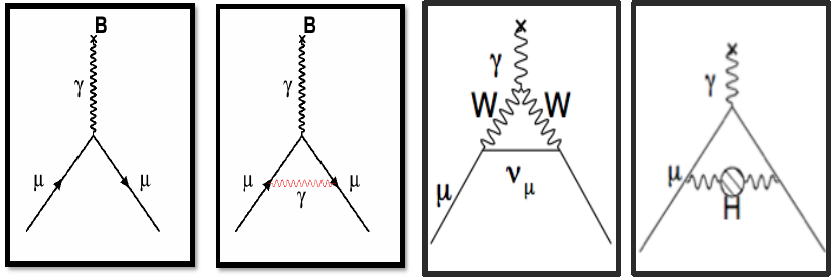
\includegraphics[width=2 cm]{a_mu_corrections.png}
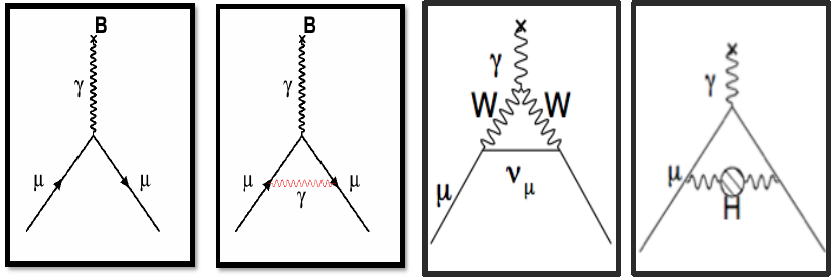
\includegraphics[width=9 cm]{a_mu_corrections.png}
%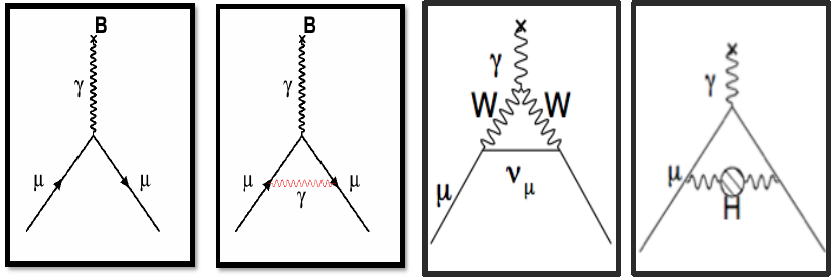
\includegraphics{a_mu_corrections.pdf}
\caption{\label{fig1}The SM correction in $a_{\mu}$ from QED, electroweak loops, HVP. }
\end{figure} 

The leading RC from the lowest order QED process from the exchange of a virtual
photon in Fig.\ref{fig1} i.e. the ``Schwinger term'', is calculated to be $a_{\mu} = (\alpha/2\pi) =$
0.00116 \cite{schwinger}. The difference between experimental and theoretical values of $a_{\mu}$
especially at sub-ppm precision, explores new physics well above the 100 GeV scale
for many Standard Model extensions \cite{benn}. 

In Fig.\ref{fig2} the yellow band represents the results of several theoretical calculations based on SM
($a_\mu = [116591802\pm49]\times 10^{-11}$ \cite{davier} with a precision of 420 ppb) 
and the blue band represents the latest experimental result from  the previous
Brookhaven E821 experiment combined with the experimental error ($a_\mu^{E821} = [116592089\pm63]\times 10^{-11}$ \cite{benn})
which shows a difference of 3.6 $\sigma$ between theory and experiment. 
This could indicate several possible models or any new model. These new models can be generally illustrated
using a relation discussed in \cite{ Czarnecki} in which new physics (N.P.) contributions scale as \cite{Dave} 
$\delta a_{\mu}(N.P.) =\mathcal{O}[C(N.P.)] \times ( m_{\mu}/M)^2 $ where M is the N.P. mass
scale and C is the model's coupling strength, related to any N.P. contributions to the muon
mass, $C(N.P.) \equiv (\delta m_{\mu}(N.P.)/\delta m_{\mu} )$.
\begin{figure}[H]
\centering
%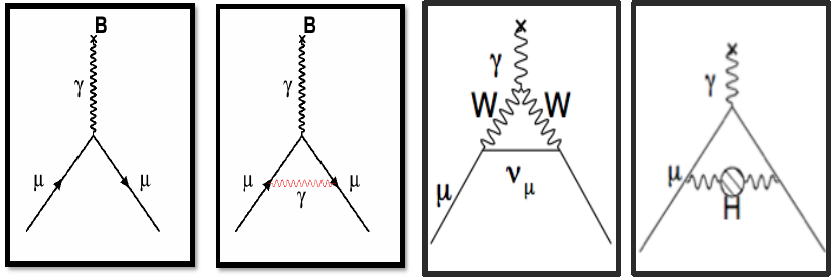
\includegraphics[width=2 cm]{a_mu_corrections.png}
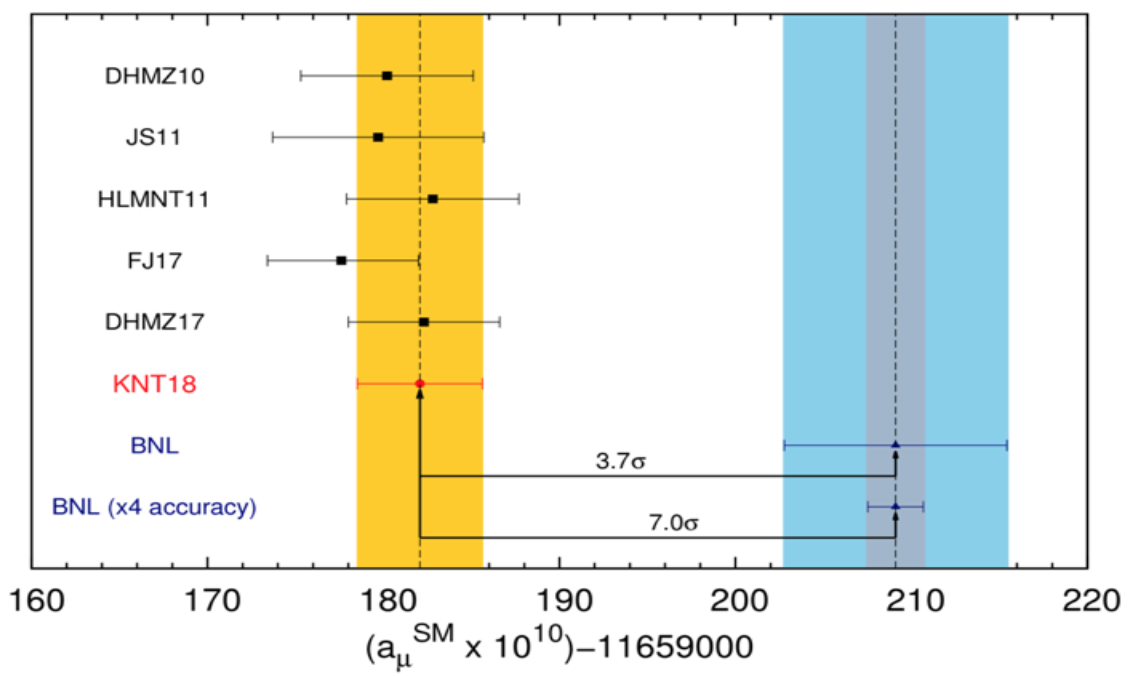
\includegraphics[width=9 cm]{comp_theory_expt.png}
%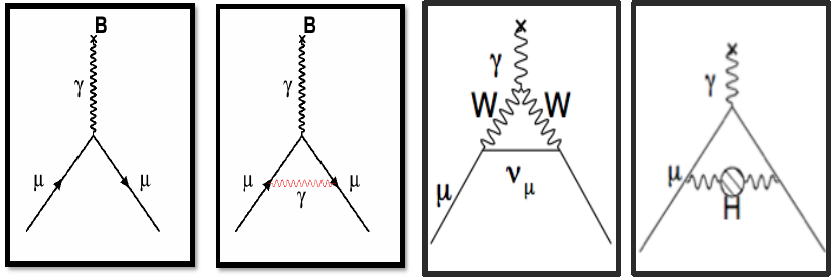
\includegraphics{a_mu_corrections.pdf}
\caption{\label{fig2}Comparison between theoretical and experimental results.}
\end{figure} 

In the multi-TeV scale, a muon mass is generated by radiative effects. %(shown in green in Fig.\ref{fig3}). 
The other possible models could be due to Z$'$, W$'$, universal extra dimensions,
littlest Higgs assume a typical weak-interaction scale coupling \cite{Dave}. %(shown in red in Fig.\ref{fig3}).
The other possibilities can represent 
unparticles, extra dimension models or SUSY with enhanced coupling \cite{Gorringe}. 
The existence of dark photons or dark $Z$ \cite{Davoudiasl:2012ig} from very weakly interacting and very 
light particles would correspond to a narrow band in the 10 - 100 MeV
mass range, having an extremely small coupling can also be possible. 
Improved precision of measurement in $a_{\mu}$ to 140 parts per billion will continue to
constrain or validate the energy scale of the models, which is the goal of ``The E989 
Muon g-2 Experiment''. This requires 21 times more statistics than the previous
Brookhaven E821 experiment and a threefold reduction of the systematic error.
%\section{Theoretical Background and Basic Technique}
%\subsection{Muon g-2: The Basics}

\section{The measurement of muon anomalous moment: The experiment}
A polarized muon beam (from pion decay) having an energy of 3.09 GeV is injected
(through the inflector shown in Fig.\ref{fig3}) in a storage ring of uniform magnetic field of 1.45 T 
with a cyclotron frequency of $\omega_c$. At the magic momentum of 3.09 GeV/c the muon spin precession frequency 
$\omega_s$ and $\omega_c$ including the Larmor and Thomas precession are approximately given by,
\begin{equation}
\begin{aligned}
%\mathcal{L}=\frac{g}{m}\left( \bar{L} \, \sigma_{\mu \nu} \, \ell \right)
%\partial^{\nu} \, W^{\mu} \,   + h.c. \,.
&\omega{_c} = \frac{e}{m\gamma}B\\
&\omega{_s} = \frac{e}{m\gamma}B(1 + \gamma a_{\mu})\\
\end{aligned}
\end{equation}
We essentially measure the anomalous frequency $\omega_a$ which is $\omega_s$ relative to $\omega_c$
i.e. $\omega_a = \omega_s - \omega_c$. From the above equations this is given by,
\begin{equation}
\begin{aligned}
&\omega{_a} = \frac{eB}{m}a{_\mu} 
\end{aligned}
\end{equation}
In this experiment, we measure the muon anomaly $a_\mu$ using the following expression,
\begin{equation}
\begin{aligned}
& a_{\mu} = \frac {\omega_a/\omega_p} {\mu_{\mu}/\mu_p - \omega_a/\omega_p}
\end{aligned}
\end{equation}
The V-A nature of the muon decay makes it a self-analyzing process to find the muon anomalous precession  
frequency $\omega_a$. The maximum energy decay positrons are emitted in a preferential direction 
with their momenta parallel to the muon spin. These positrons modulate with a frequency of $\omega_a$ and 
this frequency can thus be extracted by counting the
number of positrons above an energy threshold (optimized for the best sensitivity) as a function of
time. The right plot of figure \ref{fig3} shows the modulated counting 
rate of positrons observed in the 2001 E821 data.
The value of $\mu_{\mu}/\mu_p$ is taken from muonic hyperfine experiment where it is measured  
at $\approx$26 ppb precision \cite{hyperfine_mu}.

\begin{figure}[H]
\centering
%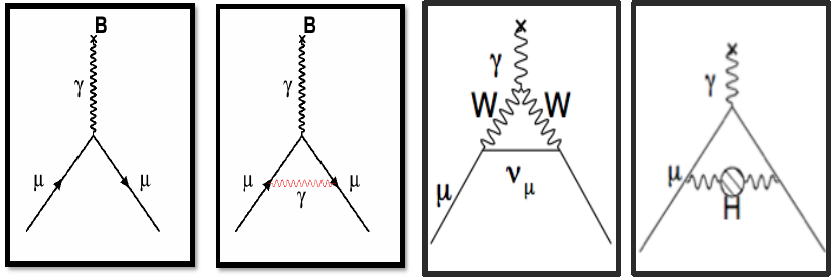
\includegraphics[width=2 cm]{a_mu_corrections.png}
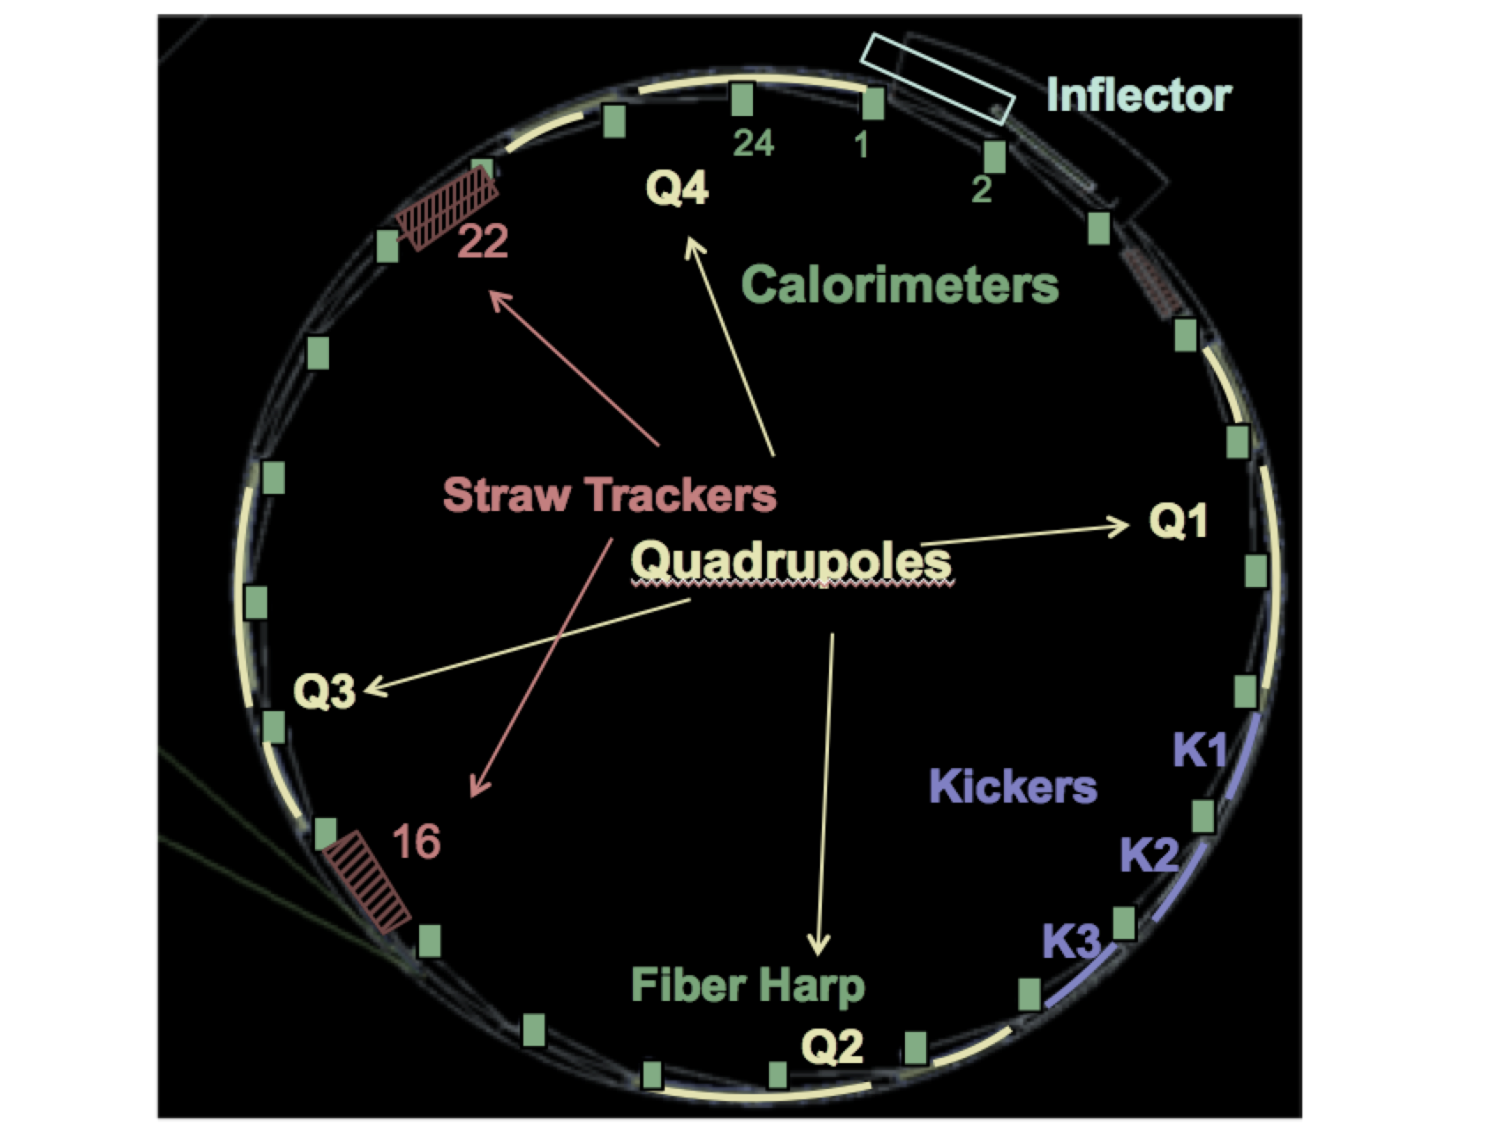
\includegraphics[width=7 cm]{ring.pdf}
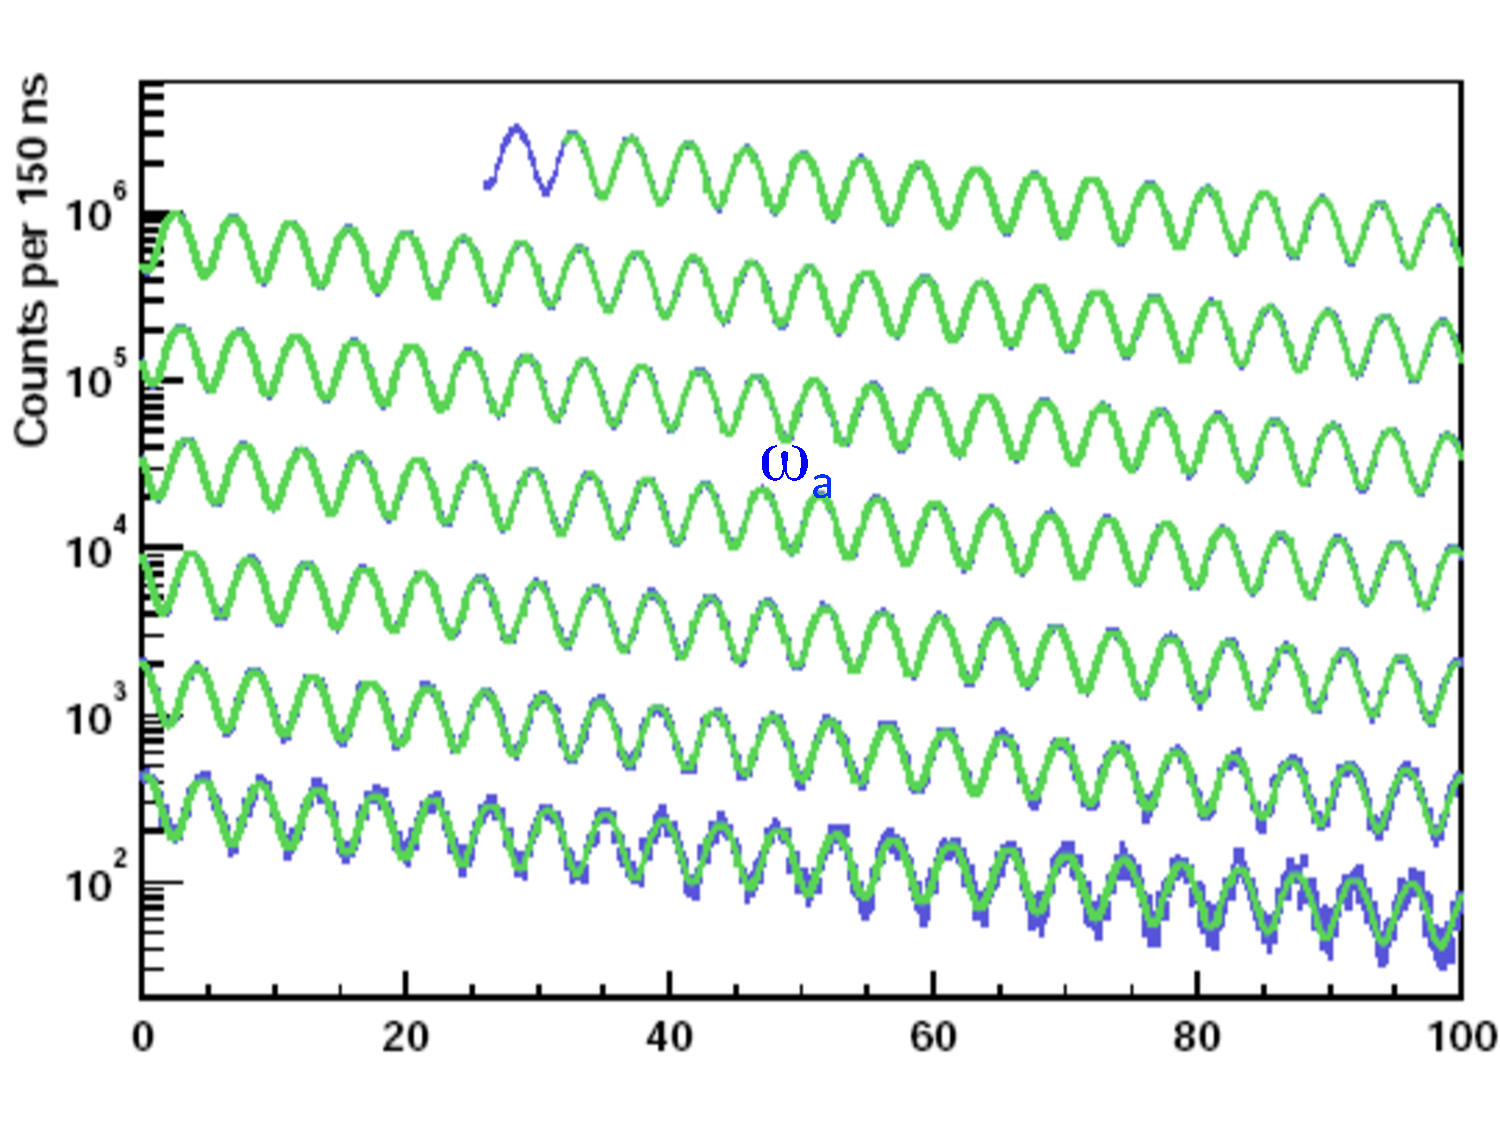
\includegraphics[width=7 cm]{wiggle_bnl.pdf}
%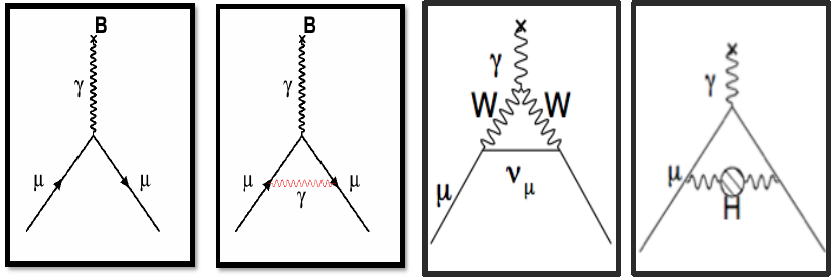
\includegraphics{a_mu_corrections.pdf}
\caption{\label{fig3}Left -- The layout of the storage ring for the E989 experiment. 
Right -- The modulated counting rate of the positron distribution of 2001 E821 data.}
\end{figure} 
The left panel of figure \ref{fig3} shows the schematic of the entire storage ring with the
kickers (K1-K3), the quadrupoles (Q1-Q4), the collimators (C), the
NMR trolley garage straw trackers and the fiber harps. The details of the 
working of each of these components will be illustrated 
in the subsequent sections. An electron calorimeter is placed at
a position indicated by the calorimeters in green numbered (1,2,...,24).
The muons decay to positrons preferentially in direction of the muon spin
which are detected by the 24 calorimeters shown in Fig. \ref{fig3}. The time spectrum
of these positrons is given by,
\begin{equation}{\label{no_muon}}
N(t) = N_0 e^{\frac{-t}{\tau}} (1 + A cos(\omega_at)) 
\end{equation}
from which $\omega_a$ is extracted. But care needs to be taken into account for the
distortions in this spectrum due to pileup, gain instabilities, beam losses, etc.

%\section{Experimental performance and comparison  with the current best measurement (E821 at BNL)}
%% OK till above
%% TO BE DONE FROM HERE
\subsection{The preparation of the Muon Beam for twenty-one times the BNL statistics}
A statistical error improvement from 540 ppb to 140 ppb (~21 times BNL) requires a
better proton beam, better $\pi$ and $\mu$ separation with an improved collection.   
This is accomplished by an 8 GeV proton produced in a booster which is then 
directed to a recycler ring further hitting an Inconel target to produce pions. 
Pions with an energy of 3.11 GeV are selected and transferred to a delivery ring with 
long decay channels (due several turns in this ring most of the pions decay 
before they reach the muon storage ring). This enables to produce polarized 
muons of energy 3.09 GeV from forward pion decays which have better spatial separated from 
pions and background protons. Thus, using a delivery ring eliminates background, 
gives a good spatial discrimination and reduces pion/proton flash. Finally, the muon 
bunches are transported to the muon storage ring in the Muon Campus 1 (MC1) experimental hall. 
An approximate run time of 18-24 months is required to acquire these statistics.  
To test all hardware equipment and installation of DAQ, DQM along with other software 
a month of the first engineering run in June 2017 took some commissioning data successfully. 
A production run 1 from the end of March to July 7th 2018 took place were we collected raw 
positron data almost twice the E821 BNL experiment.  
A new run 2 is scheduled to run from December 2018 to July 15$^{th}$ 2019. 
\subsection{Muon Beam – Focusing in Storage Ring}
As the muon beam enters the storage ring, it experiences a magnetic field from zero strength 
to the maximum value of 1.45 T, which causes it to deflect. 
The inflector magnet cancels these fringe field effects due to the main storage ring magnet, 
just before the beam enters the storage ring. It has a superconducting shield so that the
field generated by the inflector current does not affect the uniform field of the storage ring. 
A new open-ended design inflector magnet is built for E989, which prevents scattering of muons 
at the exit of the inflector which in turn will improve the muon storage efficiency.
After exiting from the inflector, the moun beam is displaced radially by 77 mm from the 
ideal orbit.  
The three kickers direct the beam onto the orbit with the help of a pulsed vertical 
magnetic field which peaks at $\approx$250 G that corresponds to a kick of about $\approx$8 mrad 
\cite{TDR}. Additionally, four electrostatic quadrupoles at 20.4 kV further enhances the radial 
focusing and enables the vertical focusing, but de-focuses horizontally. 
They are made of aluminized mylar plates and have a coverage of 
about $\approx$43\% of the circumference. The overall 
horizontal focussing is provided by the magnetic field. 
The muon beam is monitored using an Inflector Beam Monitoring System (IBMS1 and IBMS2). 
IBMS1 located just downstream of an initial time (T0) counter, consists of two planes (X and Y) of
16 cylindrical scintillating fibers of 0.5 mm diameter where the X (Y)-profile fiber pitch is 5.5 (2.7) mm. 
This is followed by IBMS2 located inside the beam injection pipe and has a similar design as IBMS1, 
except that the pitch is 3.25 mm for both planes. The two planes give the X and Y profile of the beam. 
\cite{docdb}   
%\subsection{Beam Monitoring System}
\subsection{Further improvements and checks in the current run}
A few additional detectors were installed to improve beam monitoring during kicking and 
scrapping phases and to investigate the effect of coherent betatron oscillations. 
These were mainly the fiber harps, T0, IBMS, and the straw trackers. 
The fiber harp system and the straw trackers are both needed to determine
the stored muon beam distribution. %, which must be known to make the electric field and
%pitch corrections. 
In run 1 a single harp was used to study behaviour of the muon beam flux and the
horizontal and vertical oscillatory effects of the beam due
to an electric field at 180$^o$ near calorimeter 12 as shown in fig. \ref{fig3}.
A couple of straw trackers are installed in the 
vicinity of calorimeters 16 and 22 respectively in this current run as shown in fig. \ref{fig3}. 
%These are used to reconstruct muon beam profile from positron tracks. 
\subsubsection{Fiber Harps – Checking the beam in the current run}
The fiber harps are strung
with scintillating fibers and allow for a direct, but destructive, measurement of the
distribution of stored muons and their associated beam dynamics parameters. 
\begin{figure}[H]
\centering
%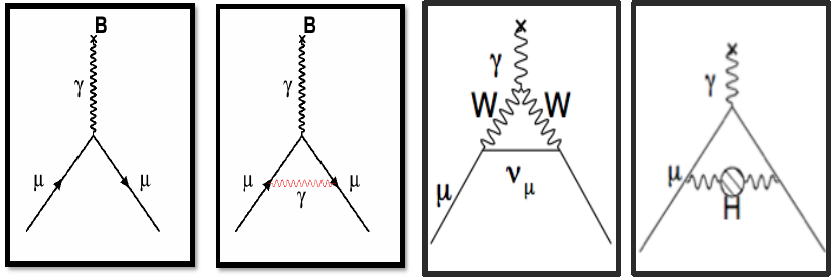
\includegraphics[width=2 cm]{a_mu_corrections.png}
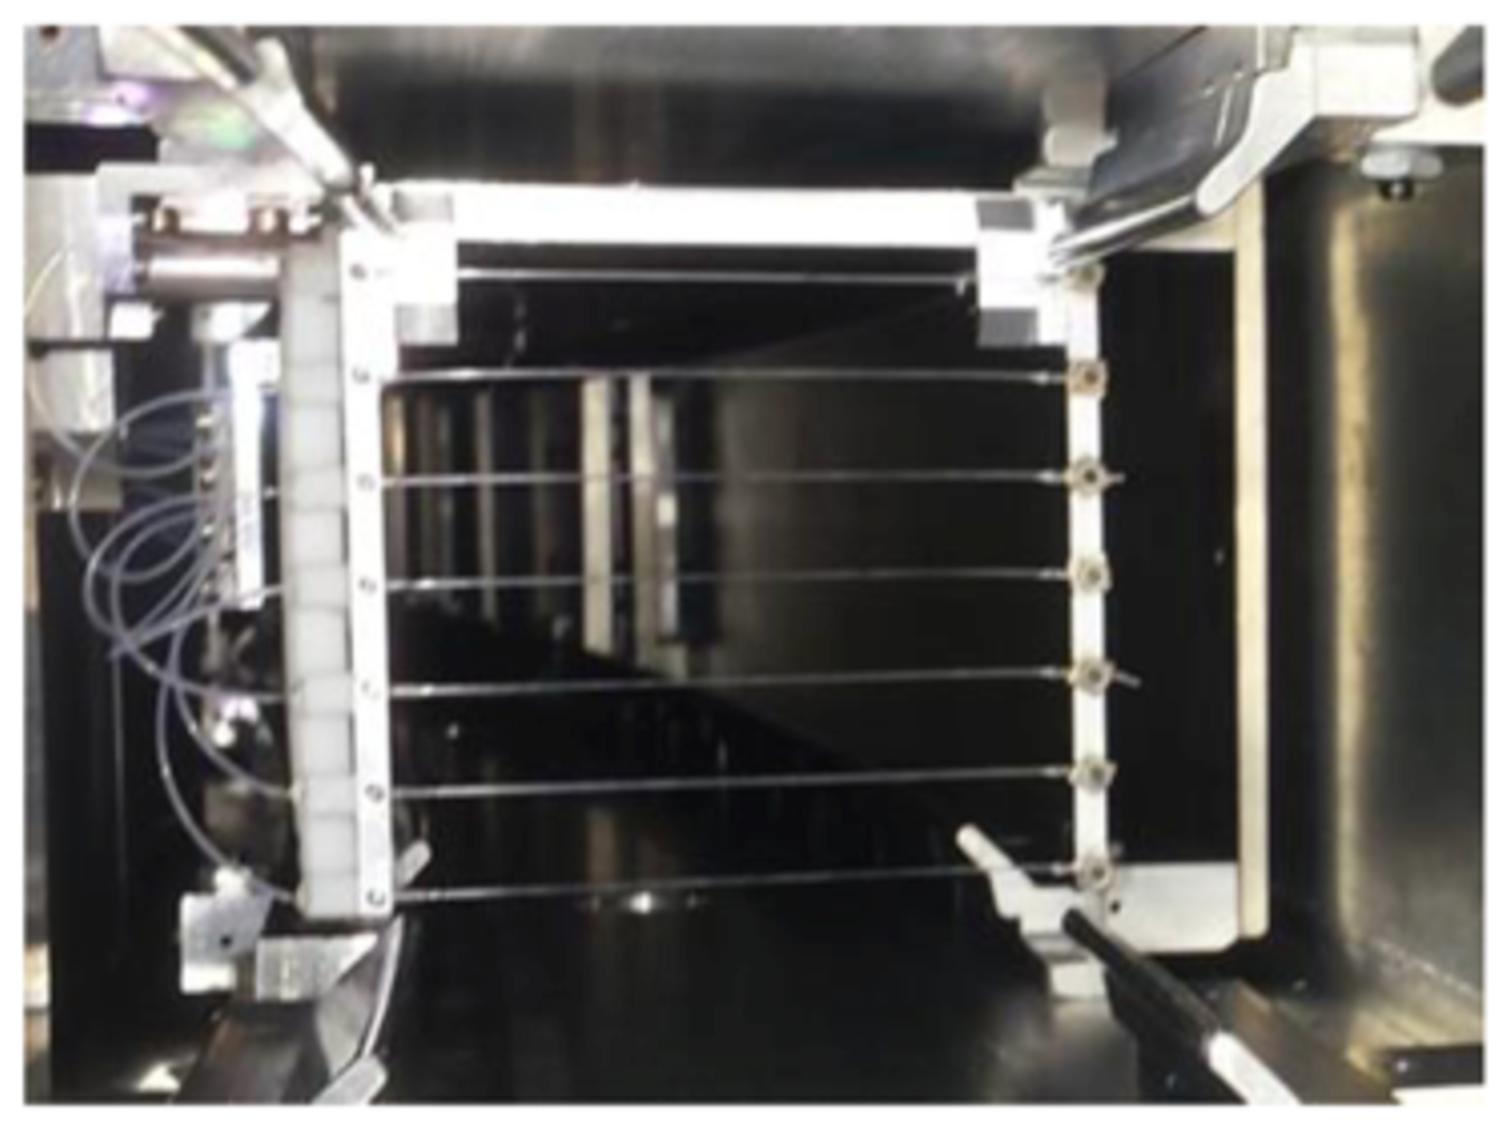
\includegraphics[width=6 cm]{harp.pdf}
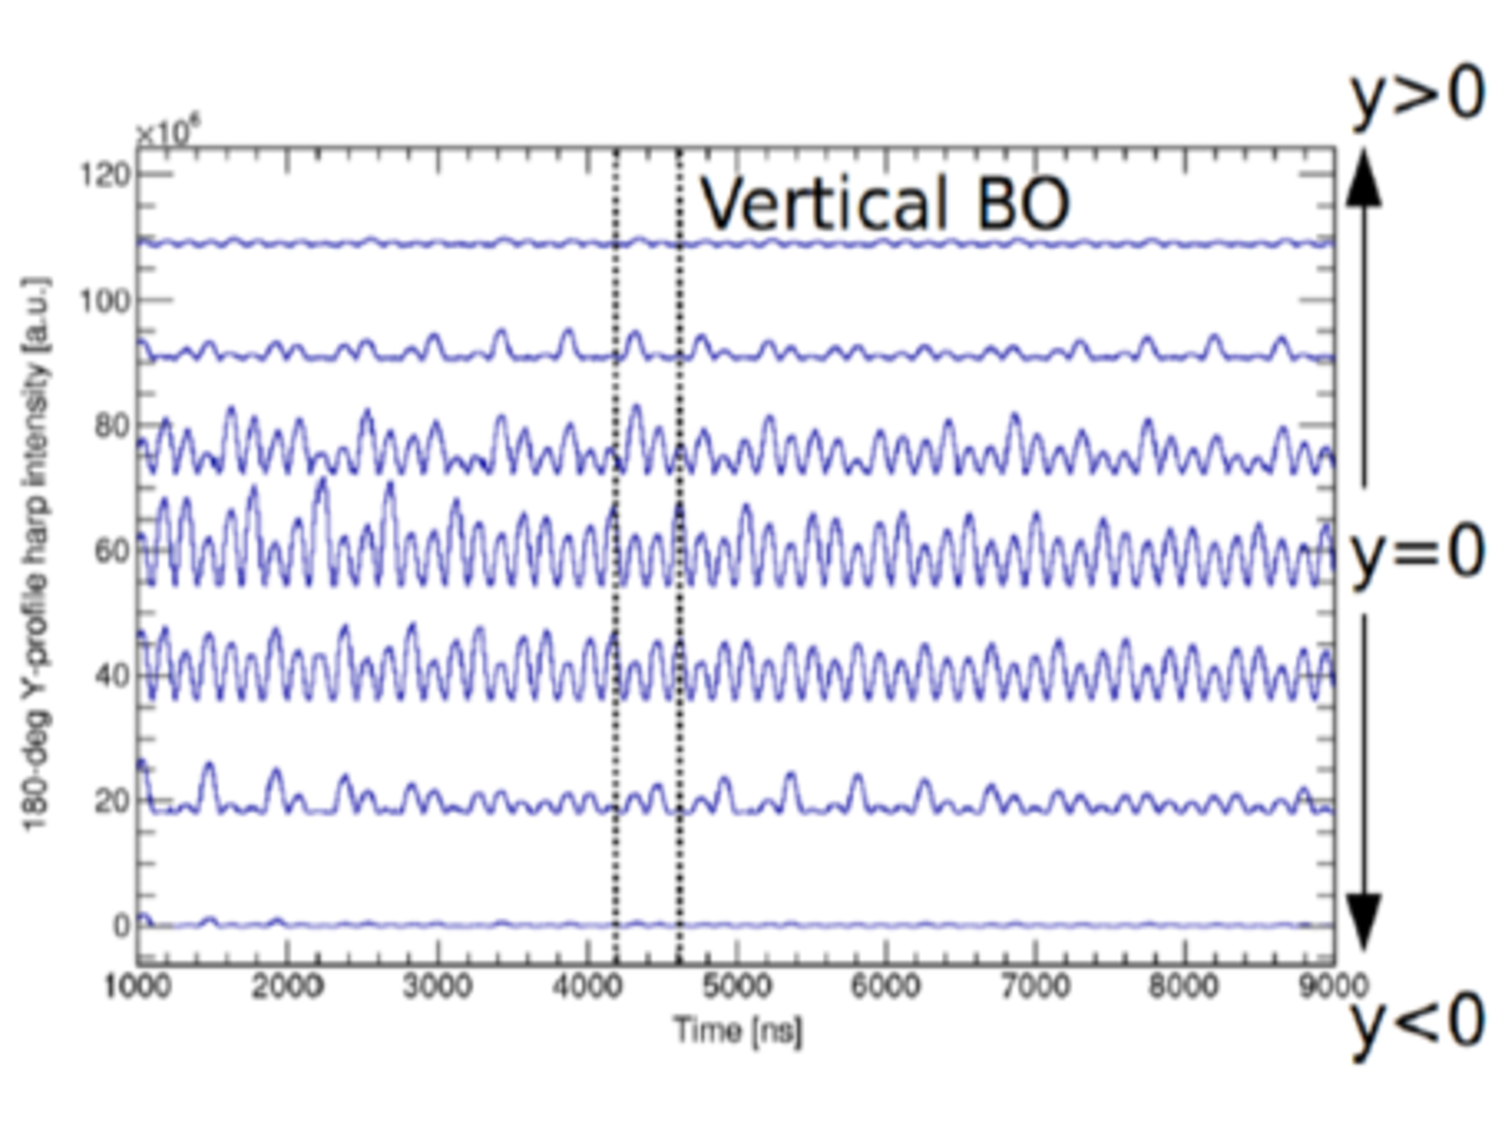
\includegraphics[width=7 cm]{vert_cbo.pdf}
\caption{\label{fig4}. The left panel is the image of a fiber harp. The right plot shows the beam 
profile in y direction measured by the fiber harp.}
\end{figure}  
%The harp is used to study behaviour of the muon beam 
%flux and the horizontal and vertical oscillatory effects of the beam due to an electric field. 
It consists of a “harp” of seven scintillating fibers of 0.5 mm diameter,
each 90 mm long and separated from its neighbors by 13 mm \cite{TDR}. 
Each scintillating fiber is further attached to a standard optical fiber as 
shown in the left image of figure \ref{fig4}. A couple of such harps were used, one suspends
the fibers vertically to measure x coordinates, and the other arranges them horizontally to measure
the y coordinates. Special fiber harp runs were occasionally taken in between data taking
(not during the actual data runs as it is an obstacle to the beam).
The left panel of figure \ref{fig4} shows the horizontal measure in y of the beam profile. 
Maximum oscillations are in the center of the beam (around y=0). This is due to 
the vertical component of the betatron oscillations. 
\subsubsection{In–Vacuum Straw Trackers}
There are two straw tube trackers installed in the ring and 
each of them consist of 8 modules with 128 straws containing Argon-Ethane (50\%) gas mixture, 
and having a resolution of 165 $\mu$m. 
Each module has two planes of straws oriented at 7.5$^o$ with respect each other, so that
both the horizontal and vertical coordinates of the trajectory can be determined.
The straws are made of 15 $\mu$m thick aluminized mylar foils with a gold-plated tungsten
wire (d=25 $\mu$m) at the center. 
\begin{figure}[H]
\centering
%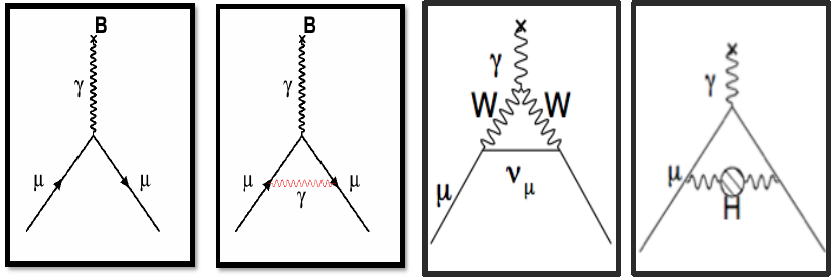
\includegraphics[width=2 cm]{a_mu_corrections.png}
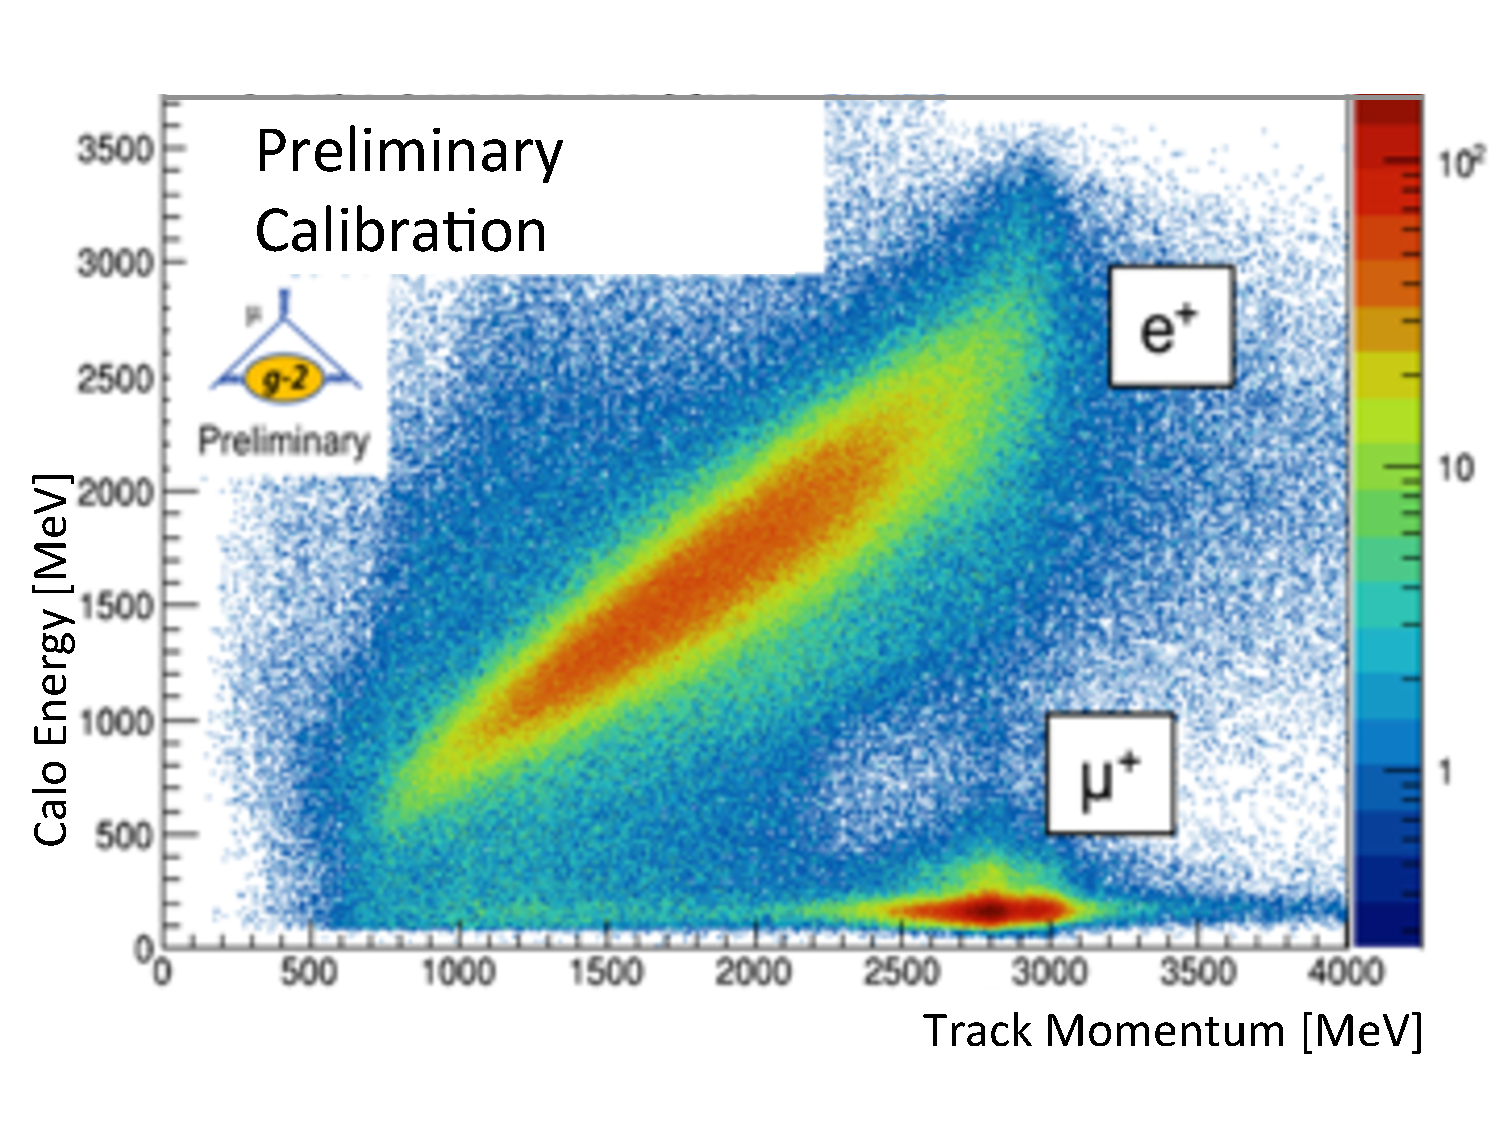
\includegraphics[width=5 cm]{track_dist.pdf}
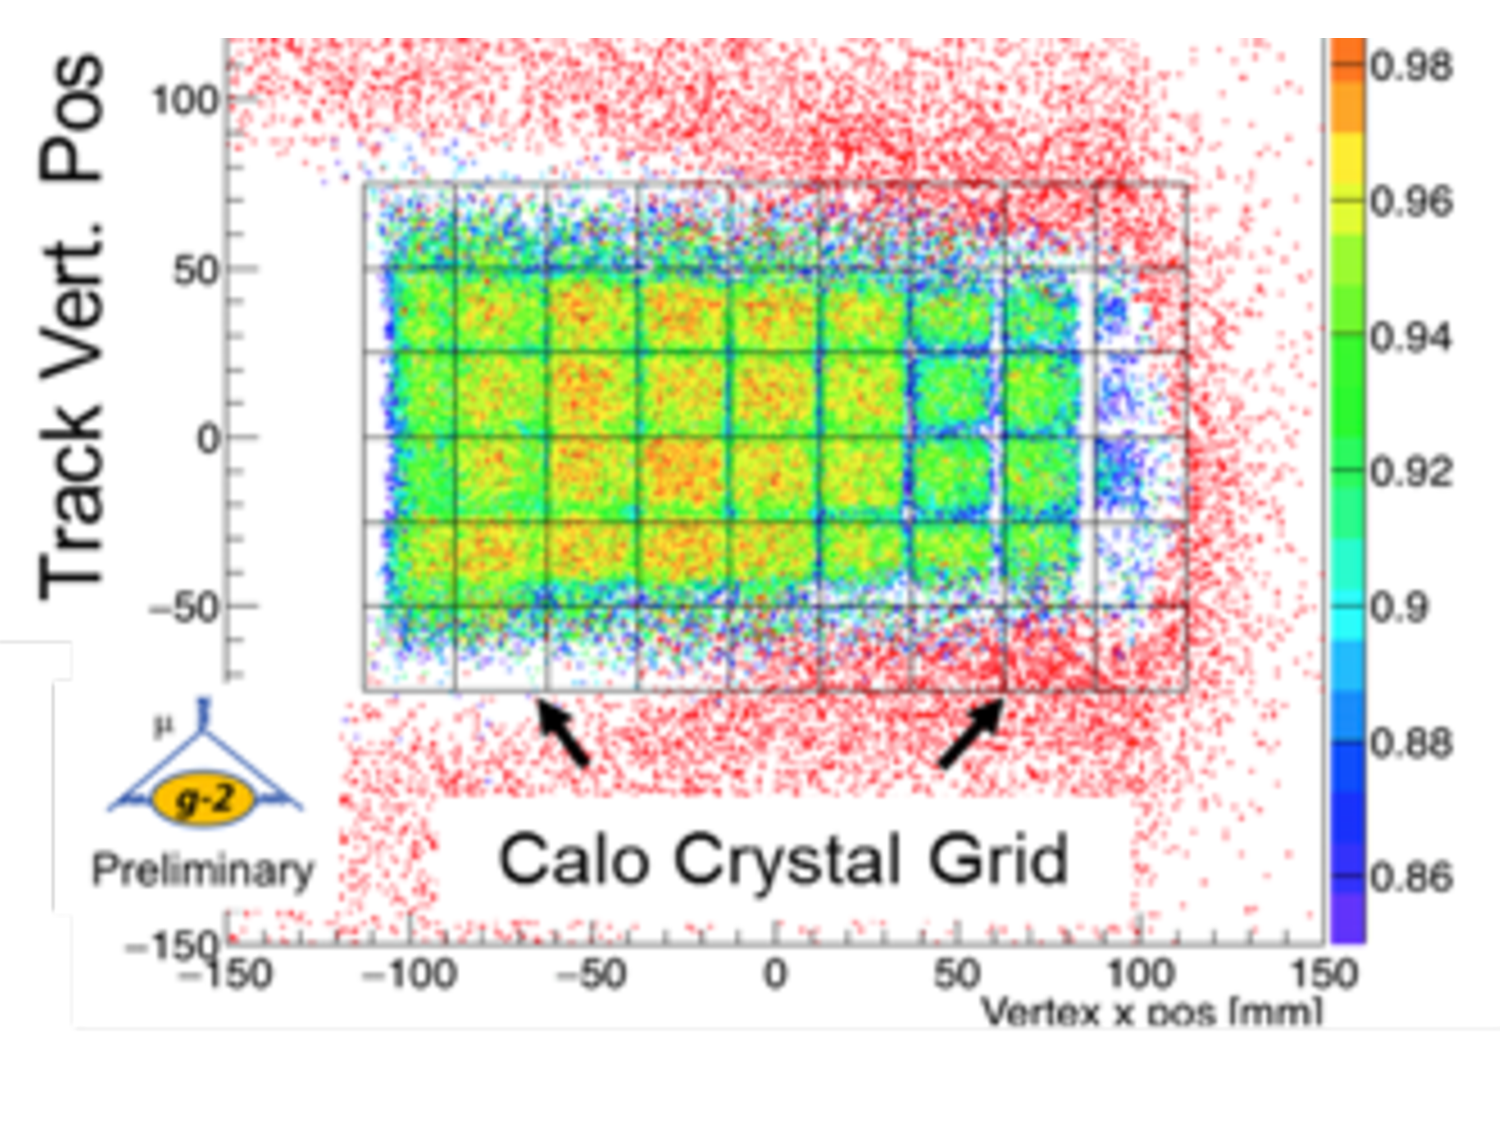
\includegraphics[width=5 cm]{calo_track.pdf}
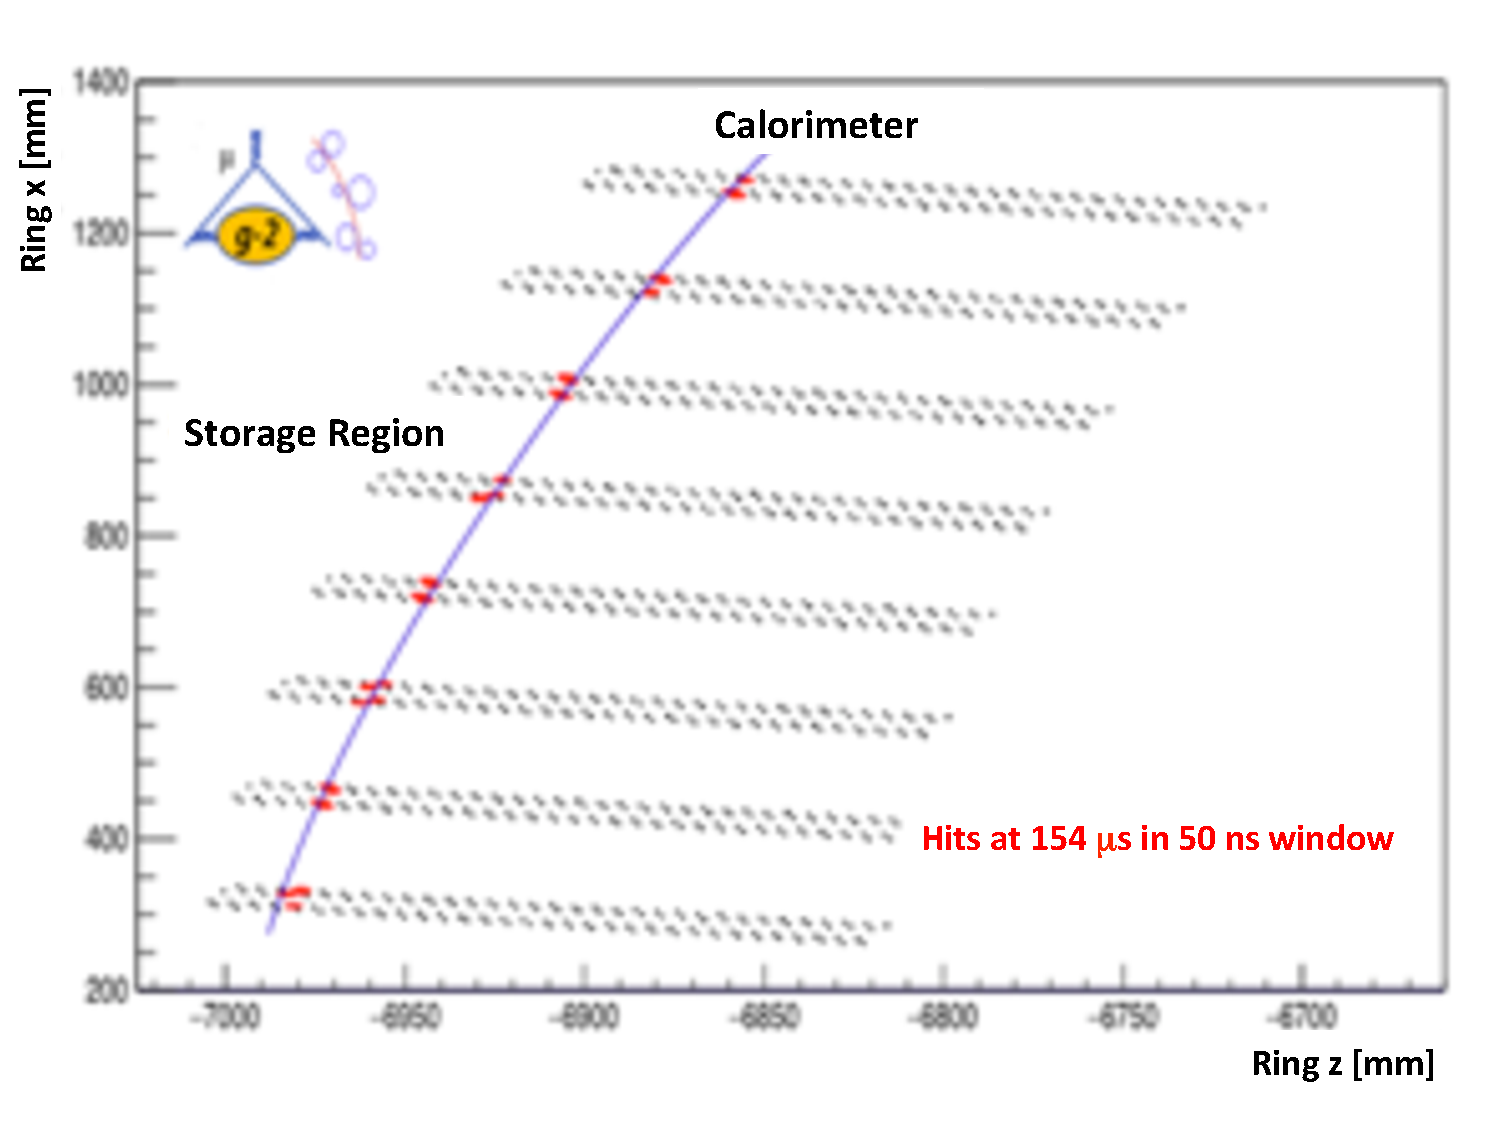
\includegraphics[width=5 cm]{tracker.pdf}
%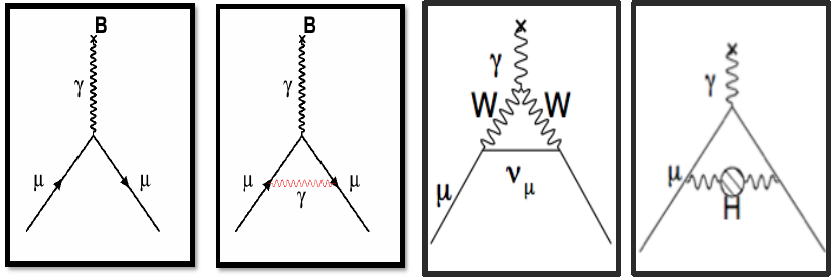
\includegraphics{a_mu_corrections.pdf}
\caption{\label{fig5}The left plot shows muon and positron discrimination from tracker data. 
The center plot shows an imaging of the calorimeters from extrapolation of positron tracks from the 
tracker. The right plot shows a positron hits in the tracker itself.}
\end{figure}  
A forward extrapolated of the track to map with the calorimeter from the
point of tangency of the ideal muon orbit allows the determination of the beam profile distribution 
(figure \ref{fig5} right). This in turn enhances a good imaging of the calorimeters 
(figure \ref{fig5} center). 
The straw trackers in combination with the calorimeters show good particle discrimination 
between positrons and muons based on the energy-momentum distribution (figure \ref{fig5} left).
\section{The Experiment – Systematic improvements}
To achieve our systematic uncertainty, it is essential to reduce the systematic uncertainties in the 
measurement of $\omega_a$ and $\omega_p$, which requires further improvement in equipment 
and other procedures related the measurement of $\omega_a$ and $\omega_p$ respectively. 
Systematics of 70 ppb on $\omega_a$ is achieved by using an improved laser calibration,
a segmented calorimeter, better collimator in the ring, and improved tracker. 
Systematics of 70 ppb on $\omega_p$ is achieved by improving
the uniformity and monitoring of the magnetic field, increasing accuracy
of position determination of trolley, better temperature stability of the magnet,
and providing active feedback to external fields \cite{wes}.
We discuss these in detail in the subsequent subsections.

\subsection{Systematic Improvements on $\omega_a$}
The table below shows the contribution to the systematics uncertainties 
of various factors on the measurement of $\omega_a$  and the proposed improvements. 
Here we emphasize the improvements in the calorimeters along with the laser monitoring system. 
\begin{table}[H]
\caption{The table shows the systematics uncertainties of various factors on the measurement of $\omega_a$ }
\centering
%% \tablesize{} %% You can specify the fontsize here, e.g.  \tablesize{\footnotesize}. If commented out \small will be used.
\begin{tabular}{lclcl}%# of columns
\toprule
\textbf{Category}	& \textbf{E821}	& \textbf{E989 Improvement Plans} & \textbf{Goal} & \textbf{Key Element}\\
&  & [ppb]  &   & [ppb] & \\
\midrule
Gain Changes	& 120	& Better laser calibration  & 20 & Laser\\
    &     & low-energy threshold &   & \\
Pileup	& 80    & Low-energy samples recorded  &  & \\ 
    &    & Calorimeter segmentation & 40 &Calo + Laser\\
Lost Muons	& 90    & Better collimator in ring & 20 & Calo + Laser\\
CBO	& 70    & Higher $n$ value (frequency) & < 30 & Inflector + Kicker\\
 &    & Better match of beamline to ring &  &\\
E and pitch & 50 & Improved tracker & 30 & Tracker\\
&   & Precise storage ring simulations &  & \\
\bottomrule
\end{tabular}
\end{table}

\subsubsection{Calorimeters}
The 24 calorimeters used to detect the decay positron spectrum are each made up of 
54(9$\times$6) $PbF_2$ crystals (for better time and space resolution which 
improves pile up separation) with Silicon Photo Multipliers (better in
enduring the magnetic field) and read out by custom 800 MSPS waveform
digitizers. 
\begin{figure}[H]
\centering
%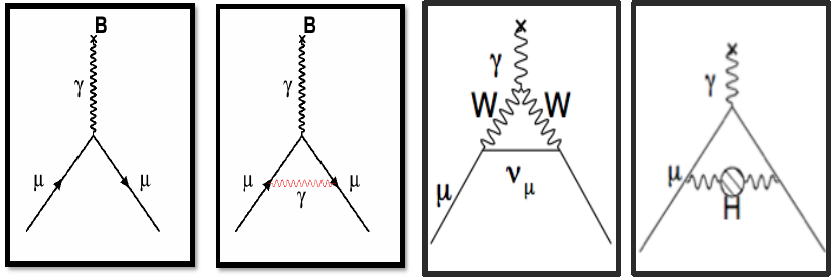
\includegraphics[width=2 cm]{a_mu_corrections.png}
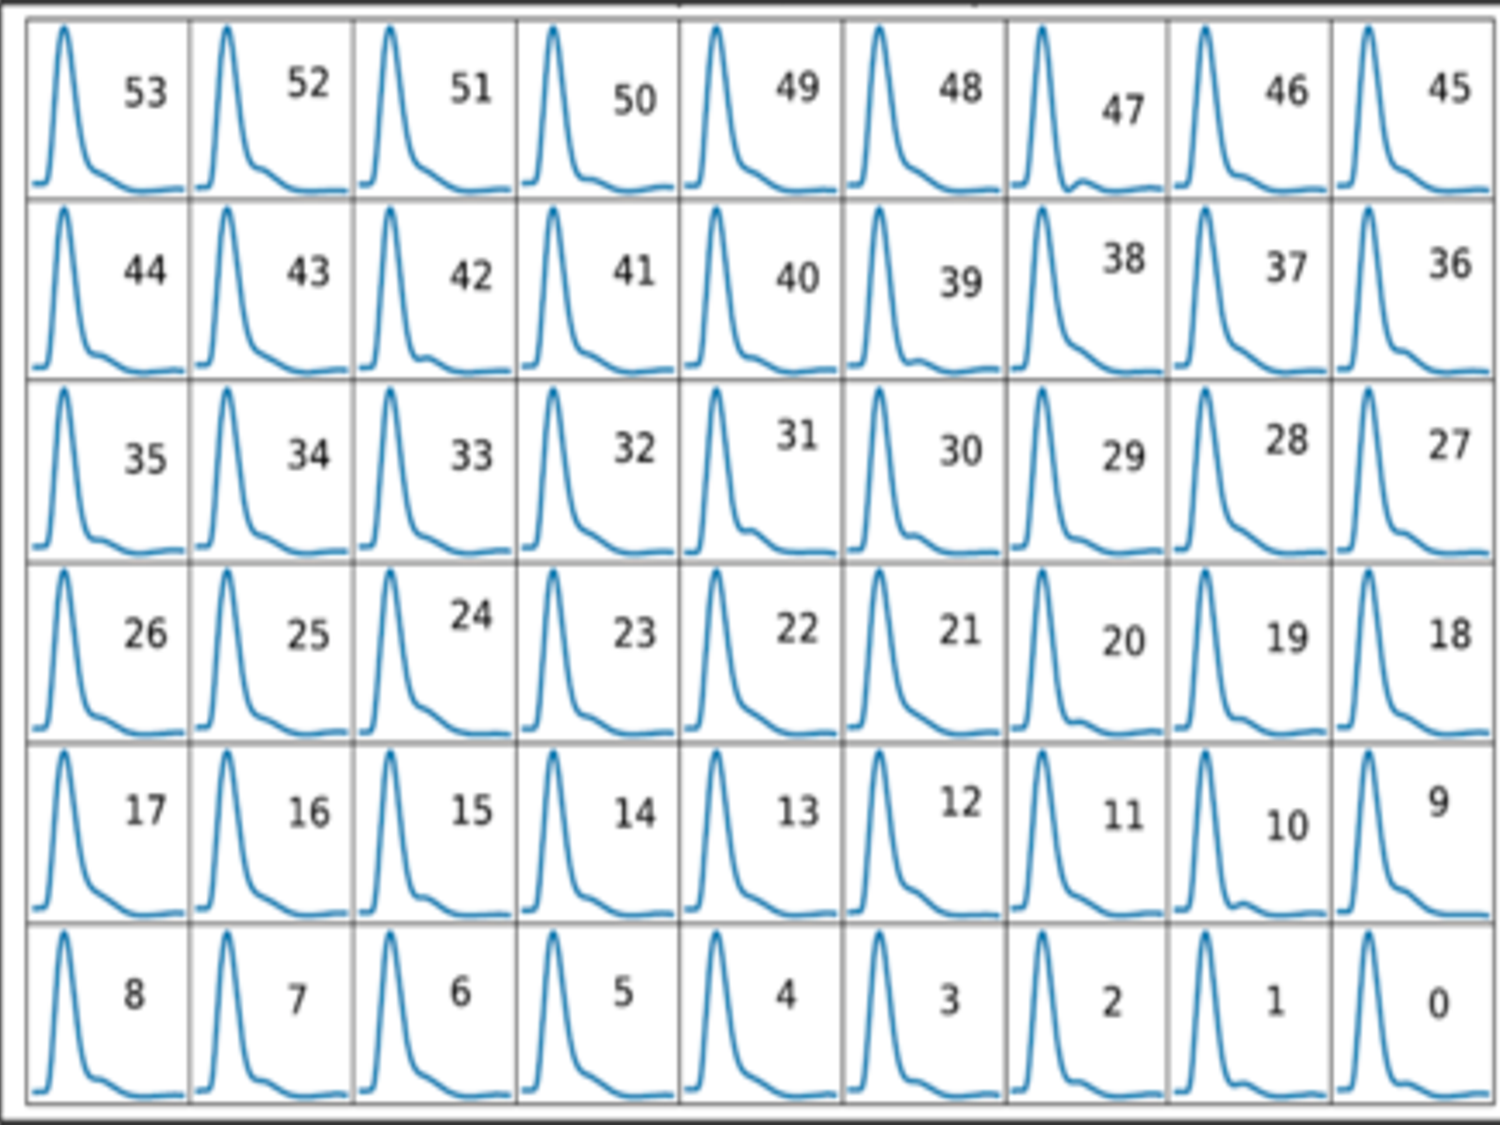
\includegraphics[width=7 cm]{template.pdf}
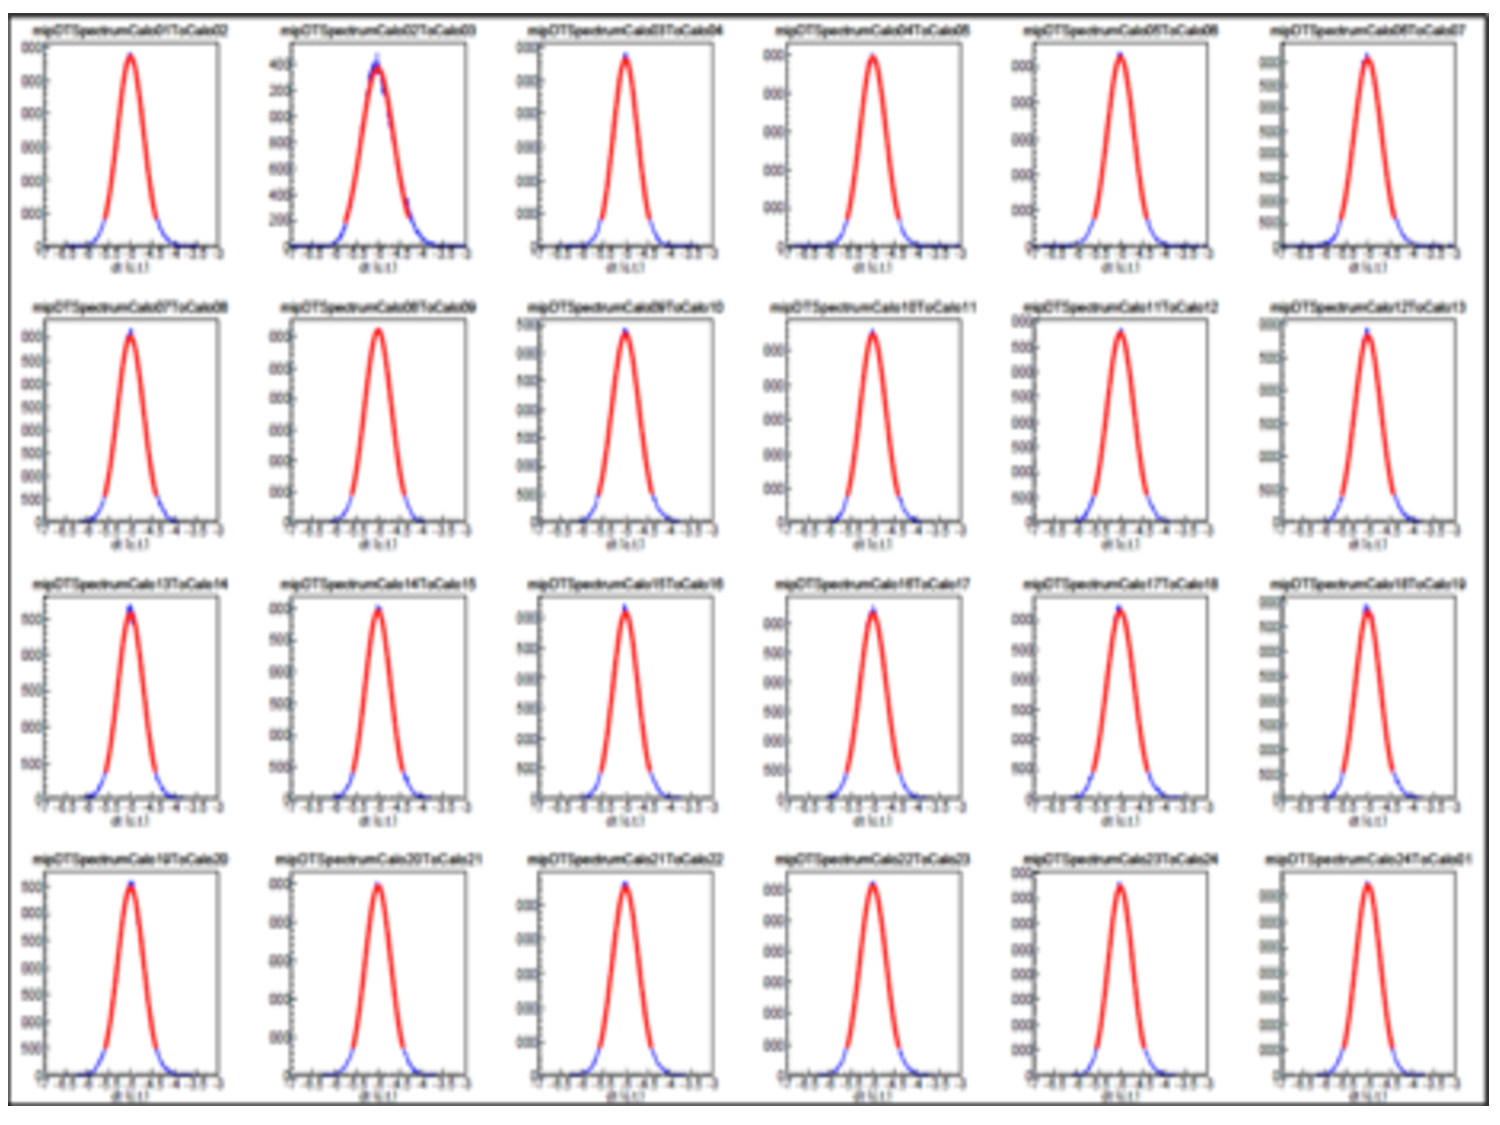
\includegraphics[width=7 cm]{time_res.pdf}
\caption{\label{fig6}. The left panel shows the custom template of all 54 crystals of a calorimeter. 
The right shows the time distribution fitted with a Gaussian for each calorimeter.}
\end{figure}
We reconstruct the pulses read by each crystal fitting a customized pulse shape (called a template) 
to the actual pulses (shown in the left panel of figure \ref{fig6}). 
The time resolution of the crystals is 25 ps at 3 GeV with a pile up separation of 4.5 ns. 
\subsubsection{Monitoring / Calibration of Calorimeter - Laser}
%check language after this...
All the 1296 crystals of the calorimeters must be calibrated and monitored to
keep uncertainties due to gain fluctuations at the sub-per mil level in the time 
interval corresponding to one beam fill (700 $\mu$s) and
at the sub-percent level on longer time scales. This is done using the laser calibration system. 
We use six laser heads (LDH-P-C-405M by PicoQuant) that provide up to 1 nJ of pulses 700 ps wide 
at a wavelength of 405 nm to calibrate all the calorimeters \cite{anas}.
The light from each laser is divided in a ratio of 
70:30 by a beam splitter. The 70\% light is further divided into four equal
parts and transported to the four calorimeters in
the ring using 25 m-long quartz optical fibers via a diffuser (to convert the 
Gaussian distribution of light intensity into a more uniform and flat distribution) and a fiber bundle.
\begin{figure}[H]
\centering
%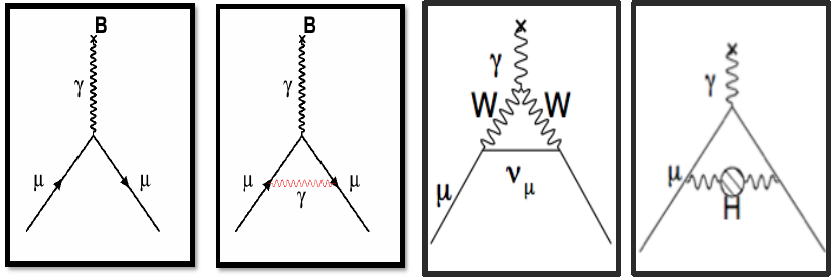
\includegraphics[width=2 cm]{a_mu_corrections.png}
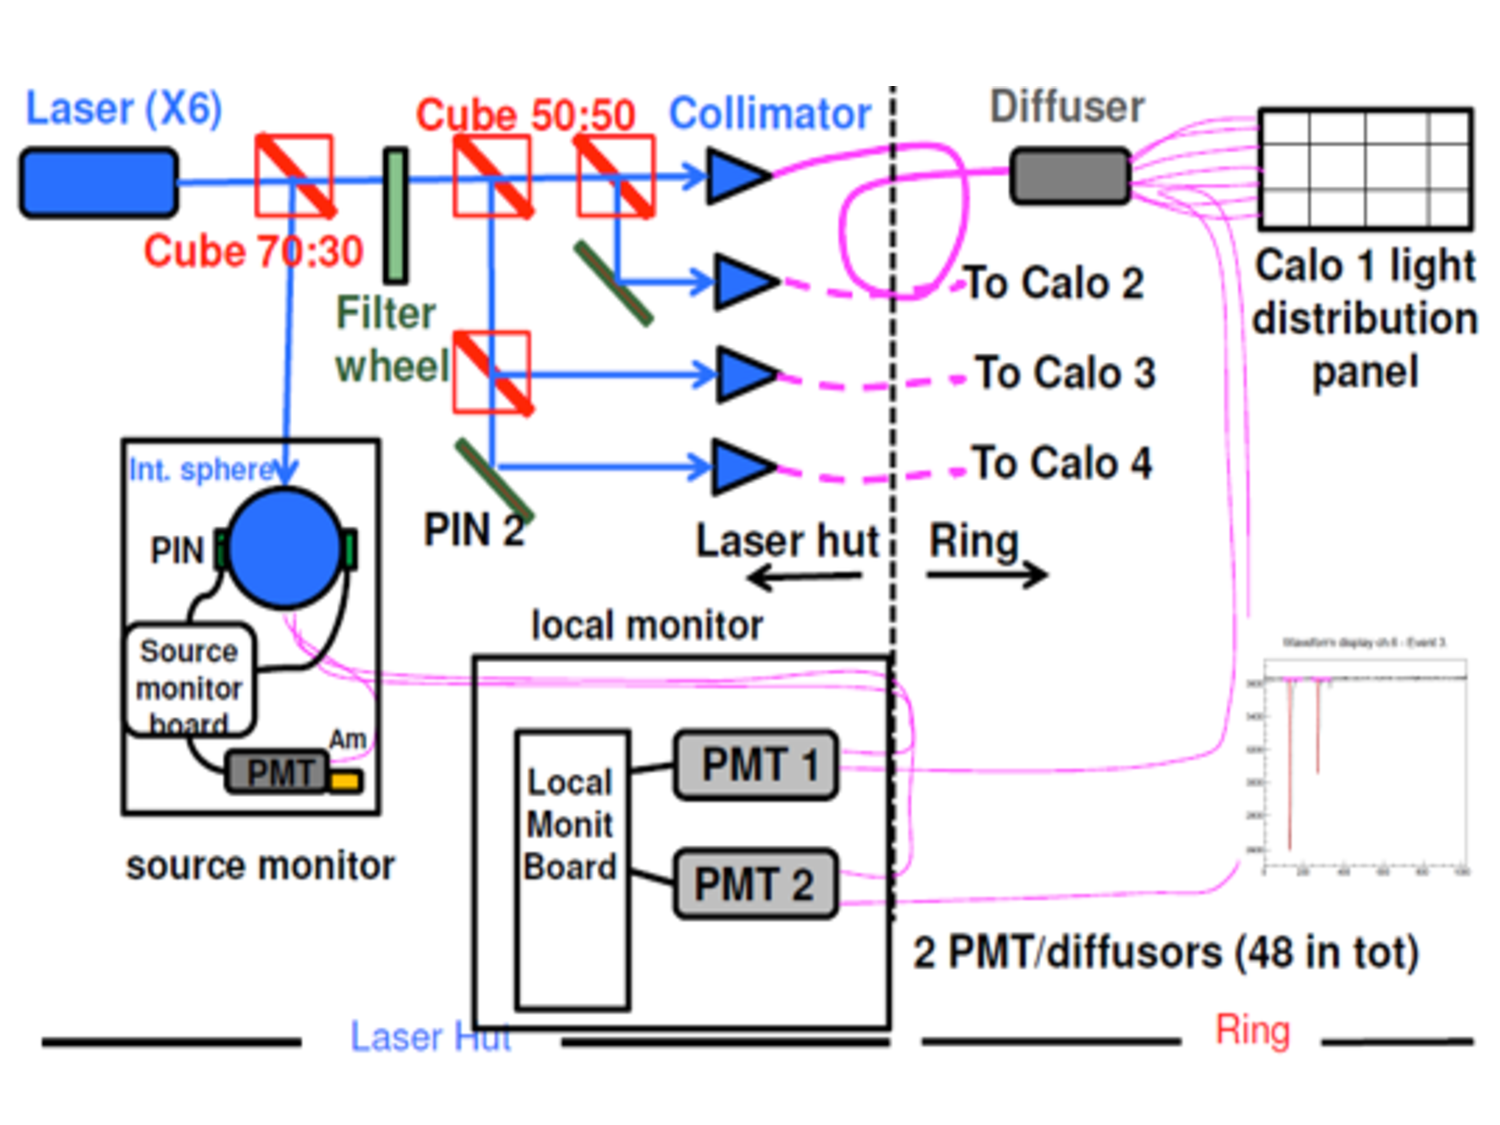
\includegraphics[width=9 cm]{laser_sys.pdf}
%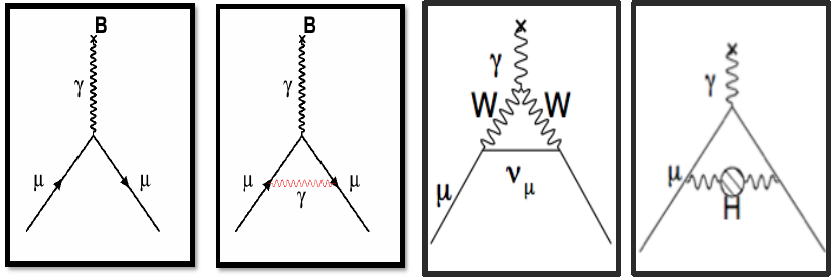
\includegraphics{a_mu_corrections.pdf}
\caption{\label{fig7}A schematic showing the laser calibration system. }
\end{figure}  
This delivers light to each of the 54 $PbF_2$ crystals with the fiber bundle attached to a 
Delrin panel embedded with optical prisms located in front of the calorimeter. 
A Source Monitor (SM) is used to measure pulse-by-pulse
the intensity of the remaining 30\% of the laser light \cite{c2}. 

The optical stability of this entire system is checked 
using 24 Local Monitor (LM). A mini-bundle fiber transmits 
light from the SM to the LM. Each LM consists of a PMT 
which collects this light from the SM and is used as a reference signal. 
The light from the optical elements, the diffuser, the 25 m quartz fiber 
(that transmits light to the calorimeter) is transmitted back to this PMT by using a quartz fiber. 
Thus, the 24 LMs are used to check the stability of the light distribution chain. 
\begin{figure}[H]
\centering
%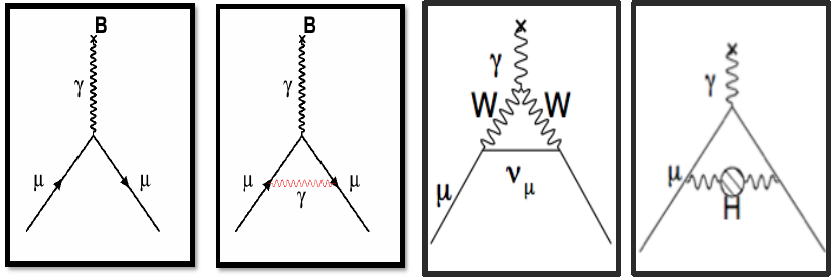
\includegraphics[width=2 cm]{a_mu_corrections.png}
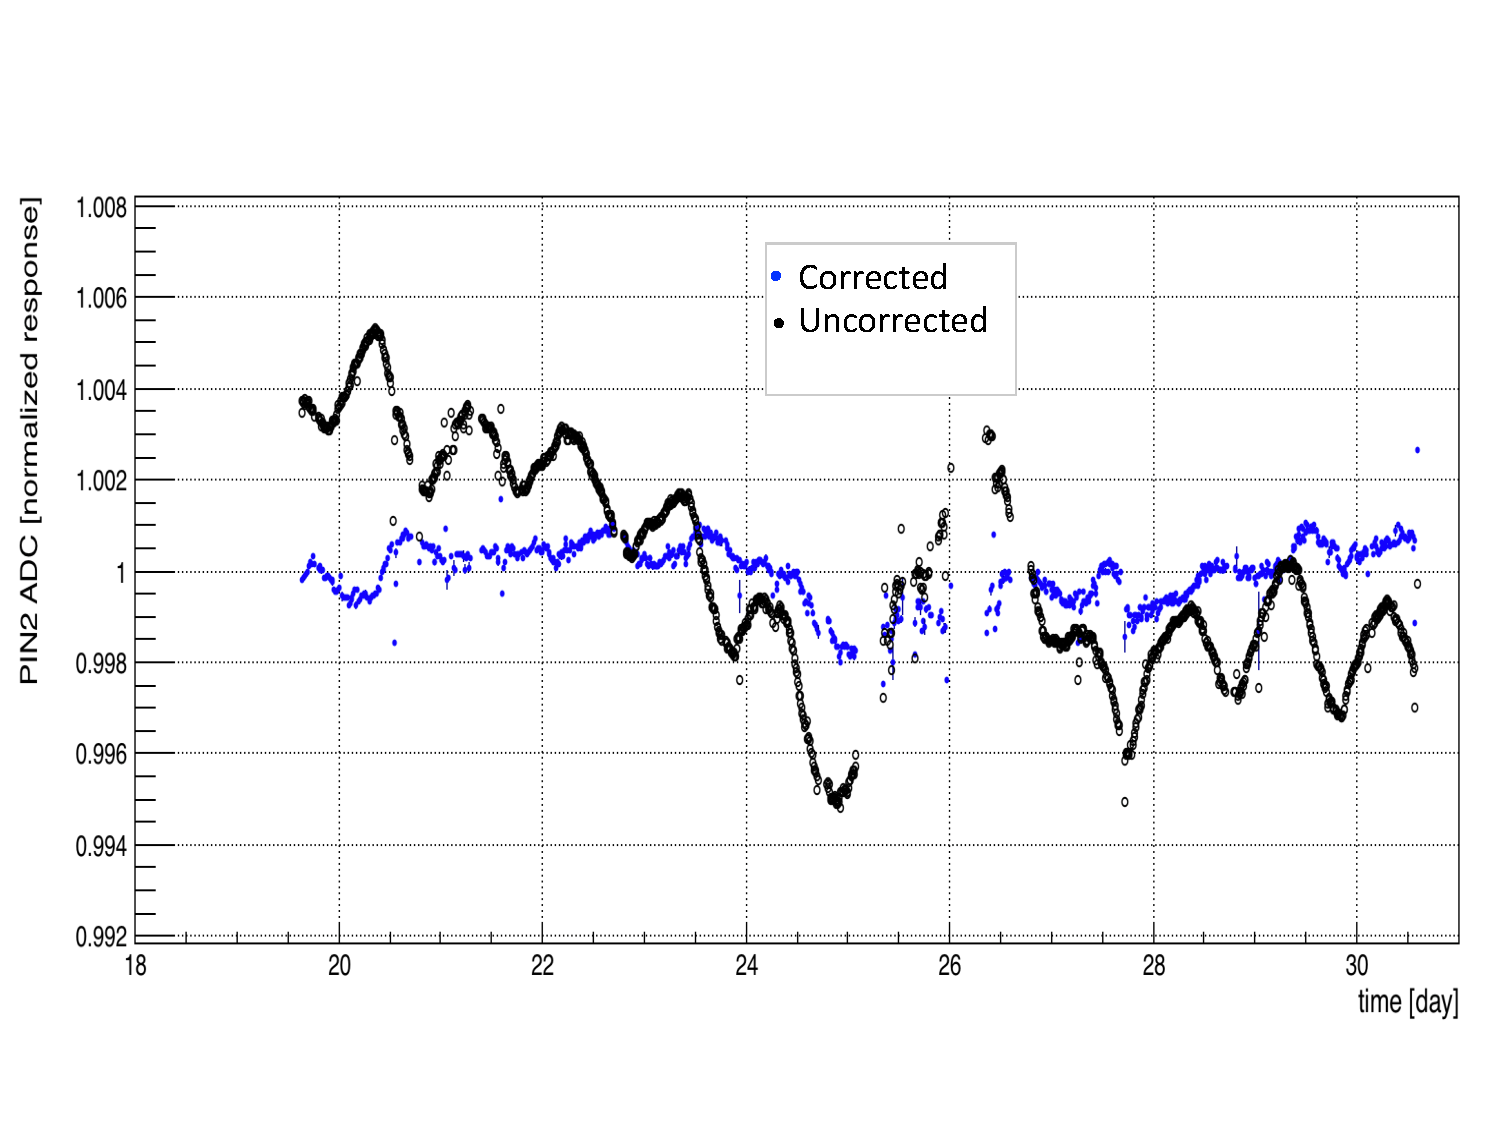
\includegraphics[width=7 cm]{SM_satbility.pdf}
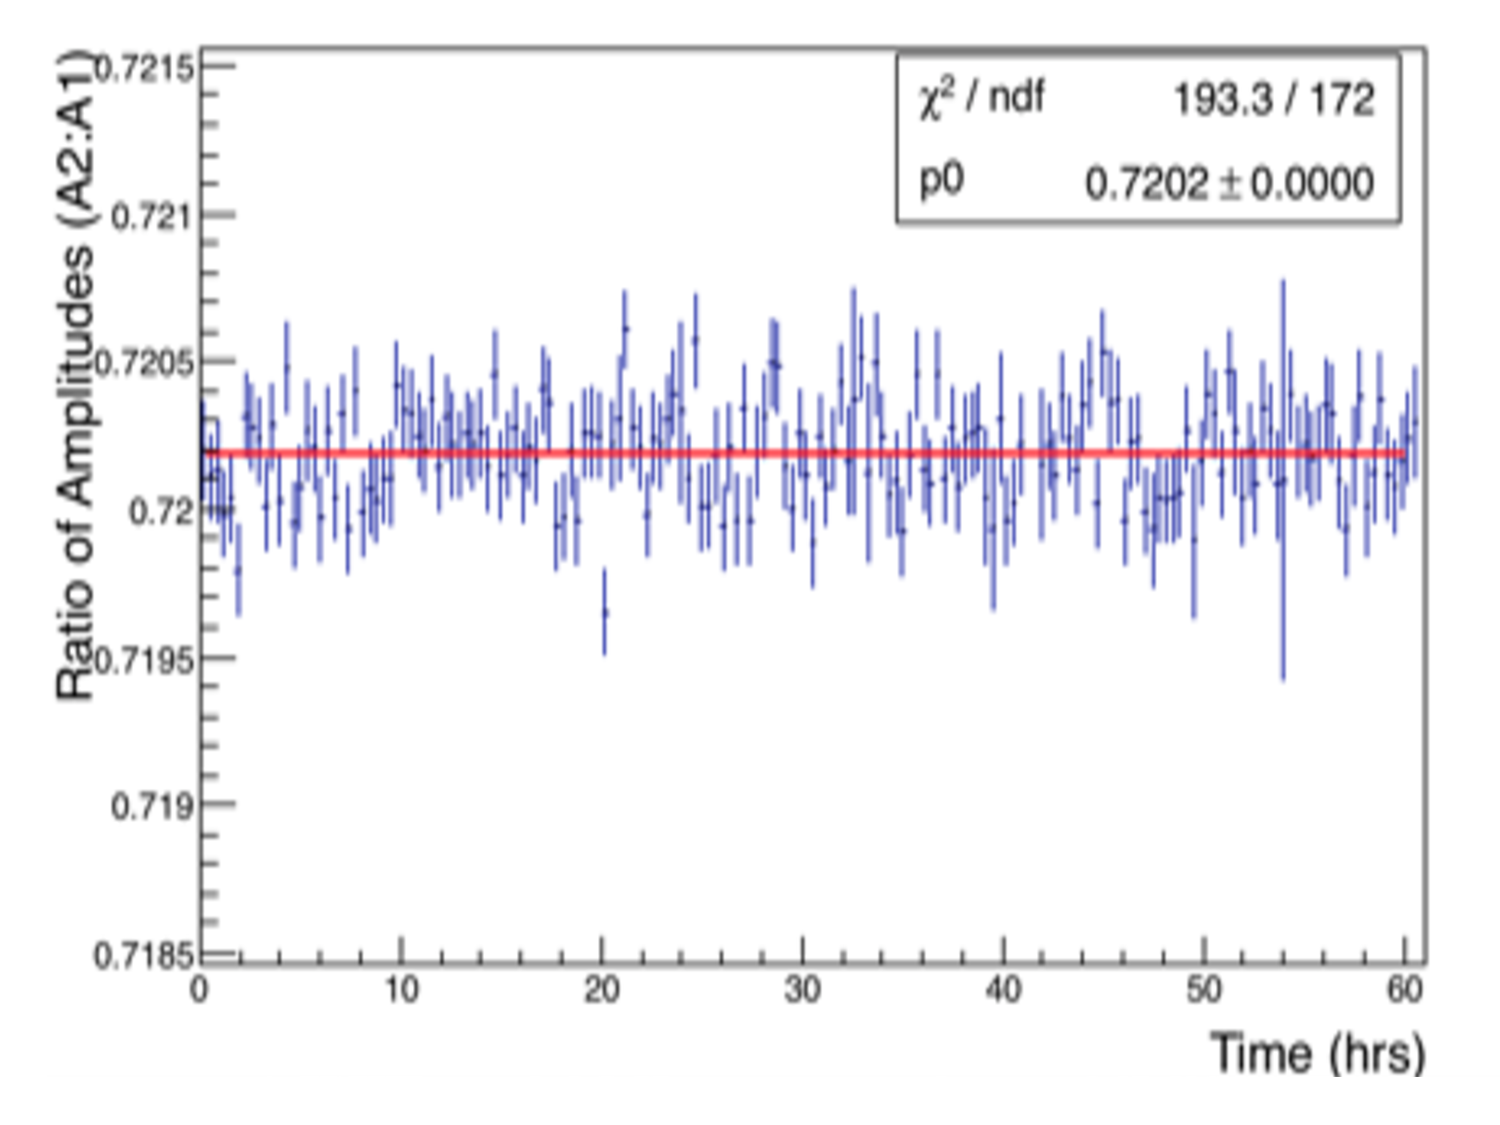
\includegraphics[width=7 cm]{LM_stability.pdf}
\caption{\label{fig8}The stabilities of the SM (left) and LM (right) after applying a temperature correction. }
\end{figure} 
Timing and gain calibrations at the subpermil level requires the system to
be very stable. After applying temperature corrections, both the SM and the LM have fluctuations of the 
order of $\approx$10$^{-4}$ (in a scale of hours) as shown in \ref{fig8}. This is reasonably good 
for the desired precision of the experiment. 
\subsection{Systematic Improvements on $\omega_p$}
As mentioned previously, the most important criteria for the improvement of systematics on $\omega_p$ 
relies primarily on the uniformity and homogeneity of the magnetic field, we briefly discuss how 
this was achieved in run 1 and the other upgrades related to this.
\subsubsection{Magnetic Field Homogeneity / Upgrade – Current Run 1}
Iron shims were used to remove asymmetries due to quadrupoles and eliminate fringe field and other stray field effects that 
distort the homogeneity of the main storage ring magnet. 
Top hats adjustments were used above the pole pieces (outside the yoke) to change the effective dipole moment.
Usage of surface correction coils and iron foils made the field more uniform. 
Using iron lamination in the current run further increased the uniformity of the magnetic field to $\plusminus$25 ppm.
\begin{figure}[H]
\centering
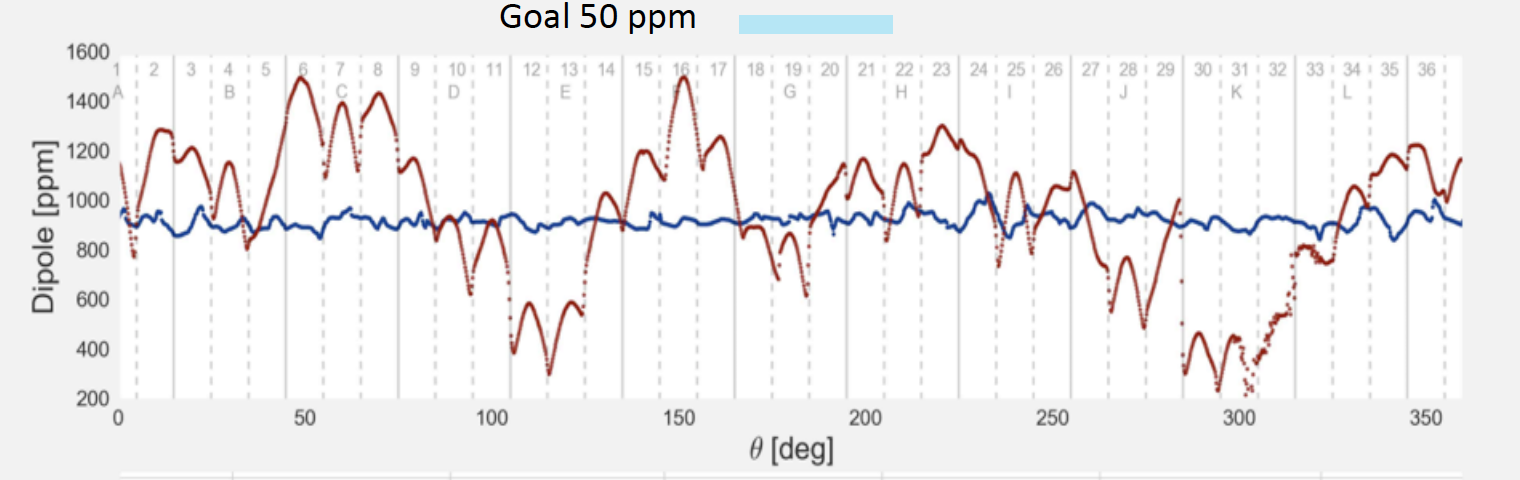
\includegraphics[width=12 cm]{shim_mfd.png}
\caption{\label{fig9}Comparison of the magnetic field before (brown) and after (blue) 
shimming, laminations, calibration etc. of the magnet. }
\end{figure} 
An absolute field calibration is also essential for reducing the systematics on $\omega_p$. 
A 1.45 T calibration magnet within a thermal enclosure (0.1$^o$C) with additional probes and better electronics 
helped in achieving this. 
Trolley probe calibrations and trolley measurements of B$_o$ need to be done with extreme care. 
Plunging probes that can cross calibrate off-central probes with a better position accuracy by physical stops 
were used to achieve this. We used 378 fixed probes at 72 locations around the ring and more than 
25 trolley calibrations run for improvements in field mapping. The results of the stability of the magnetic field due to 
shimming, laminations, and calibration are shown in blue in fig. \ref{fig9}. The brown shows the 
original field before these changes were applied. 
%Field stabilized to + 21 ppb
%\section{Measurements and systematics}
\section{Current run brief analysis status}
Several analysis techniques using various method are underway at various places simultaneously. 
The two major analysis techniques we use are called the T - method and Q - method. 
In the T - method we use the parameterization of equation \ref{no_muon} with calorimeter events 
sorted to obtain time and energy. The events vs. time-in-fill histogram (thus the name T - method) 
is built from all events with reconstructed energy above a threshold energy (1.86 GeV) and 
$\omega_a$ is extracted by fitting this equation. All events have the same weight. 
Pile up protection is essential in this method. 
This method requires a polarization of the muon beam to be above 95\% from the simulation 
and an asymmetry of A = 0.38 (refer equation \ref{no_muon}) and number of events N$_{o}$
in the fit to be 1.6 $\times$ 10$^{11}$ for a 100 ppb statistical uncertainty \cite{TDR}. 
\begin{figure}[H]
\centering
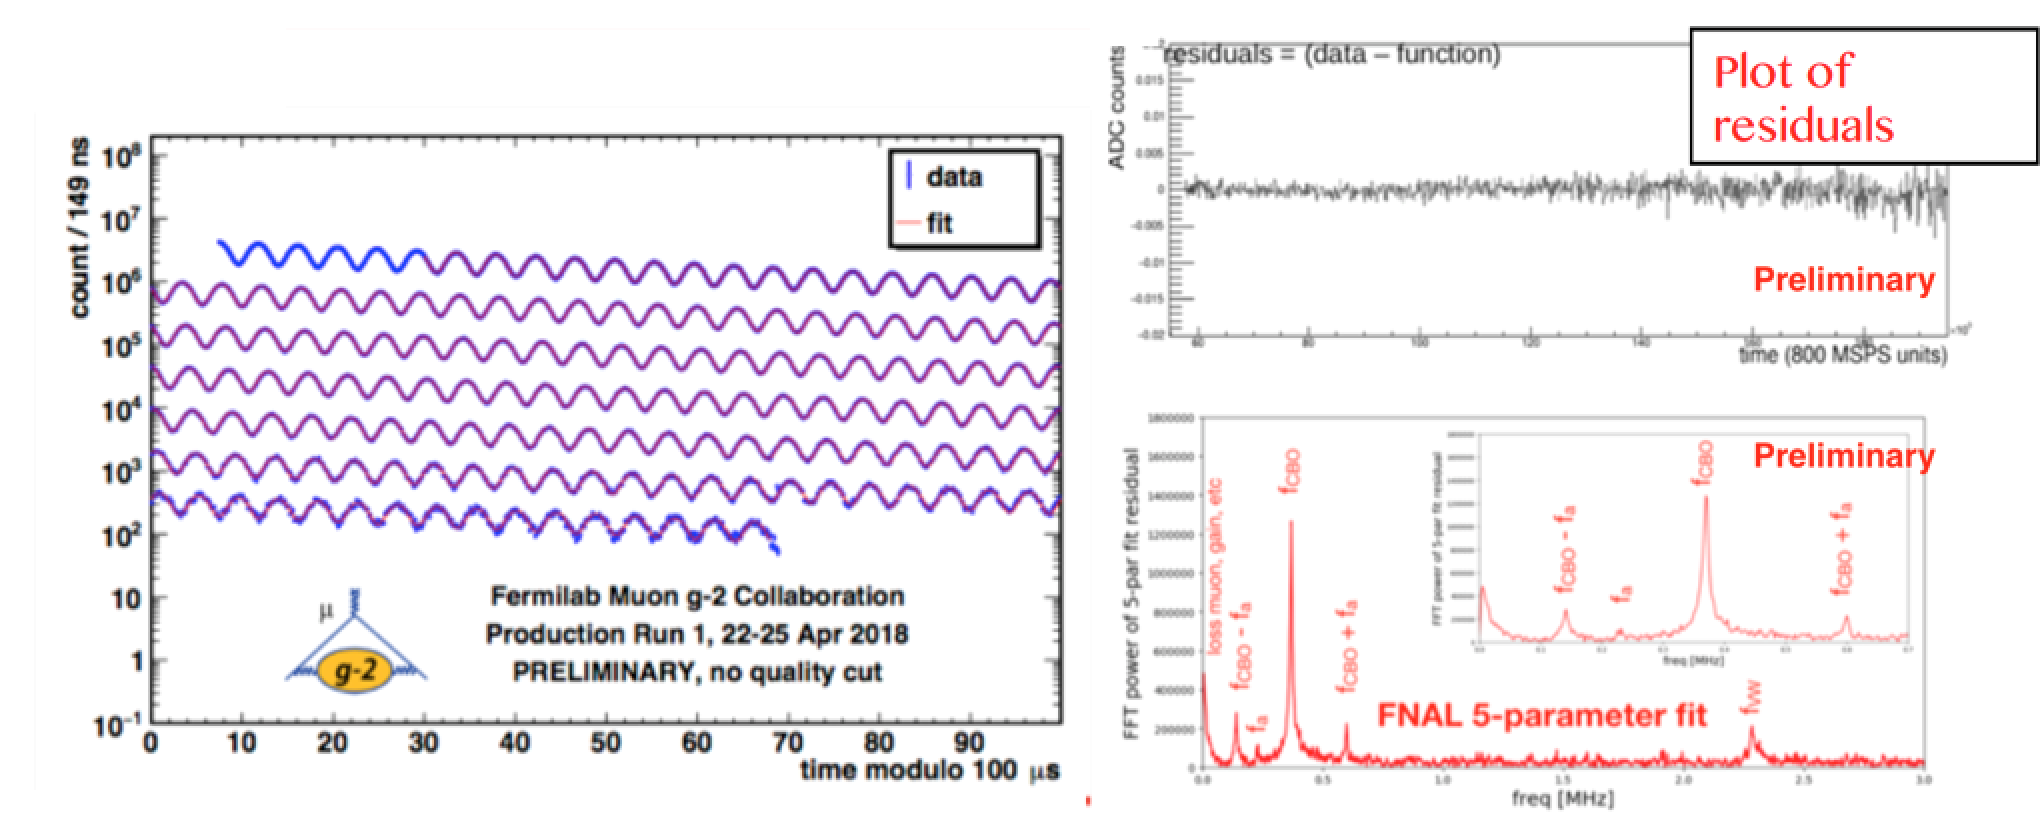
\includegraphics[width=13 cm]{analysis.png}
\caption{\label{fig10} A fit to the modulated positron distribution plot (left). A plot of residues (top right) and a Fourier transform on this (bottom right).}
\end{figure} 

In the alternative Q (charge) - method we digitize the detector current vs. time, 
which is proportional to the energy deposited in the calorimeter
vs. time from the decay positrons. All events are weighted inherently with energy 
and have an almost zero threshold. Thus, the energy in the detector will oscillate with a frequency of $\omega_a$, 
which can be fitted to determine $\omega_a$. This approach does not require pile-up protection. 
We perform a blind analysis in both cases with an offset (in clock frequencies and data) so that there 
is no bias on the analysis results. 
A fitted  modulated positron distribution plot with T-method on a dataset 
of run 1 is shown in the left panel of figure \ref{fig10} 
A plot of the residues is shown in the top right panel of figure \ref{fig10}. A Fourier transform on the residues 
plot shows structures due to CBO effects ($f_{CBO}$), vertical oscillations ($f_{vw}$), muon losses (or other effects). 

\section{Results and conclusion}
In run 1 we were able to achieve performance improvement in 
beamline, injection, and detector systems compared to BNL E821. 
A significant improvement in systematics was also achieved as discussed before. 
The data quality was good enough to find a signature of $\omega_a$, but with the current 
rate of positrons per fill we will achieve a factor of two lower positron events than the ideally 
anticipated case (as shown in the left plot of figure \ref{fig11}). 
\begin{figure}[H]
\centering
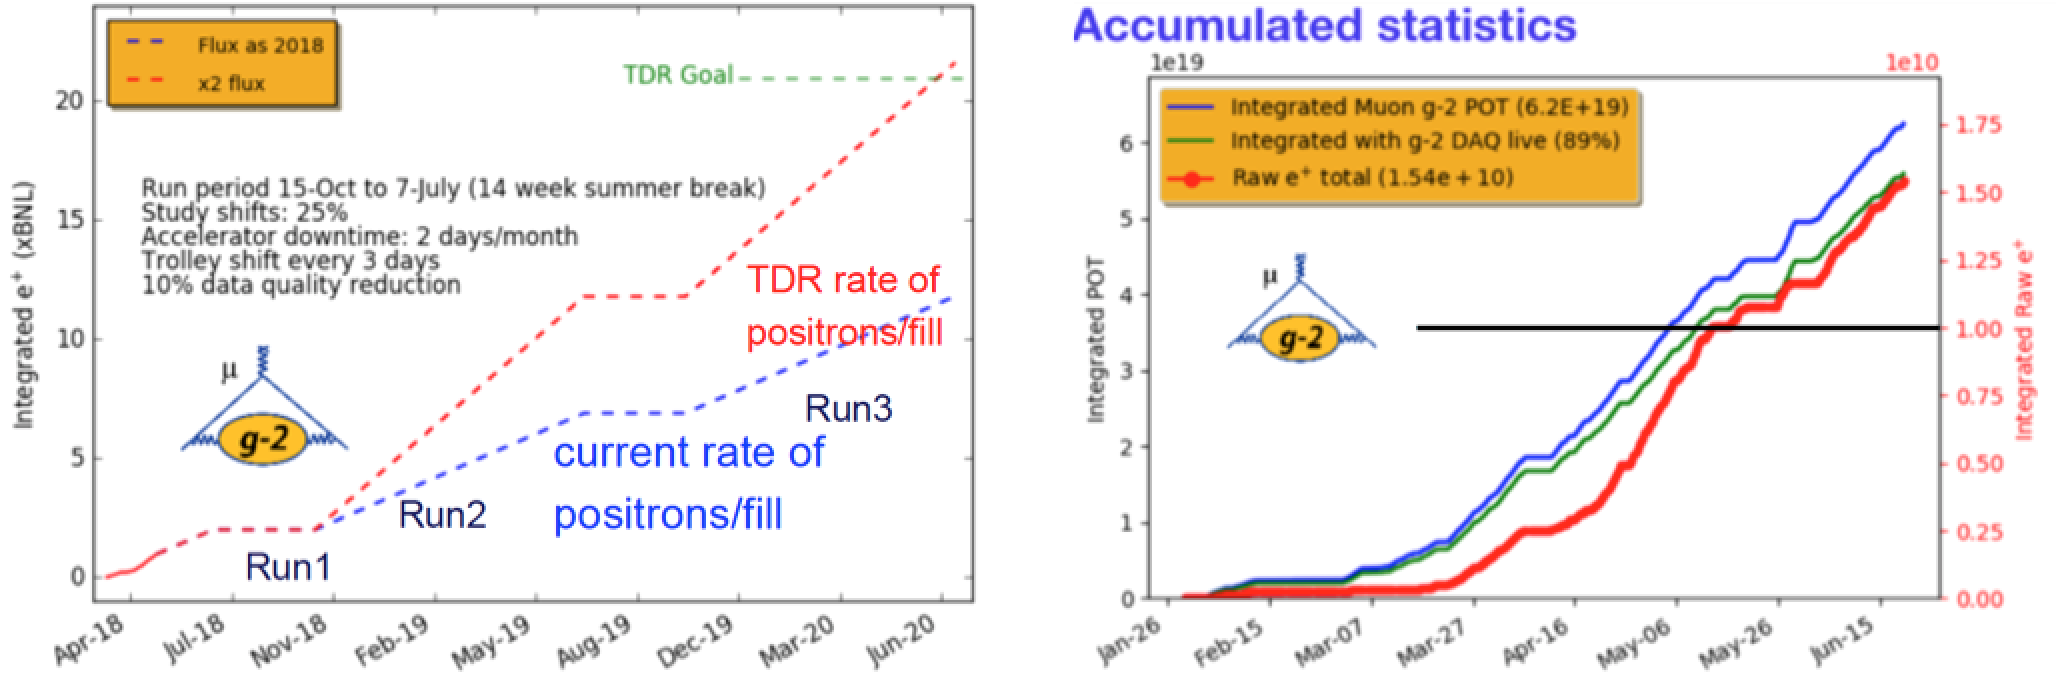
\includegraphics[width=11 cm]{statistics.png}
\caption{\label{fig11} The left plot shows accumulated statistics of integrated positrons with a future projection. 
The right plot shows accumulated statistics of POT (protons on target) in blue and the raw number of positrons in red for the current run.}
\end{figure} 
In this run we accumulated statistics $\approx$2 times the BNL experiment. 
After applying quality cuts for reconstruction of data, the accumulated statistics is the same as that 
of the BNL experiment. An analysis of this data is expected to be done by the second half of 2019 
which will verify (or disprove) the previous result. 
In a few years we expect to improve the uncertainty to 140 ppb in the measurement of $a_{\mu}$.
If the previously measured value of $a_{\mu}$ is confirmed, then we can have 7$\sigma$
discrepancy from SM, which will be a firm indication of physics beyond the Standard Model. 
\vspace{6pt} 

%%%%%%%%%%%%%%%%%%%%%%%%%%%%%%%%%%%%%%%%%%
\funding{This research was funded by Instituto Nazionale di Fisica
Nucleare (Italy), by Fermi Research Alliance, LLC under Contract
No. DE-AC02-07CH11359 with the United States Department
of Energy, and by the EU Horizon 2020 Research and
Innovation Program under the Marie Sklodowska-Curie Grant
Agreement No.690385 and No.734303.}

%%%%%%%%%%%%%%%%%%%%%%%%%%%%%%%%%%%%%%%%%%
%\acknowledgments{In this section you can acknowledge any support given which is not covered by the author contribution or 
%funding sections. 
%This may include administrative and technical support, or donations in kind (e.g. materials used for experiments).}

%% optional
%\abbreviations{The following abbreviations are used in this manuscript:\\

%\noindent 
%\begin{tabular}{@{}ll}
%RC & Radiative Correction\\
%QED & Quantum Electrodynamics\\
%HVP & Hadronic Vacuum Polarization\\
%SM & Source Monitor\\
%LM & Local Monitor\\
%\end{tabular}}


%%%%%%%%%%%%%%%%%%%%%%%%%%%%%%%%%%%%%%%%%%
% Citations and References in Supplementary files are permitted provided that they also appear in the reference list here. 

%=====================================
% References, variant A: internal bibliography
%=====================================
\reftitle{References}
\begin{thebibliography}{999}
% Reference 1
\bibitem[J. Schwinger(1948)]{schwinger}
J. Schwinger, {\em Phys. Rev.} {\bf 1948}, {\em 73}, 416.
 % Title of Schwinger paper On Quantum-Electrodynamics and the Magnetic Moment of the Electron.
\bibitem{benn}
G.W. Bennett, et al. {\em Phys. Rev. D73:072003}, {\bf 2006}.
\bibitem{davier}
Davier et al. {\em Eur. Phys. J. C 71, 1515}, {\bf 2011}.
\bibitem{Czarnecki}
A. Czarnecki and W. J. Marciano, {\em Phys. Rev.}, {\bf 2001} D64, 013014
\bibitem{Dave}
D. Hertzog, {\em Ann. Phys (Berlin)} {\bf 2015}, courtesy D. Stockinger
\bibitem{Gorringe}
T. P. Gorringe and D. W. Hertzog, {\bf 2015} doi: 10.1016/j.ppnp.2015.06.001
\bibitem{Davoudiasl:2012ig}
 H.~Davoudiasl, et al. {\em Phys.\ Rev.\ D} {\em 86}, {\bf 2012} 095009
\bibitem{TDR}
J. Grange, et al. Fermilab. Muon (g-2) Technical Design Report: -FN0992-E.
\bibitem{hyperfine_mu}
Peter Mohr, et al. {\em Rev. Mod. Phys. 84, 1527-1605},{\bf 2012}, arXiv:1203.5425 [physics.atom-ph]
\bibitem{docdb}
Website: \url{https://gm2-docdb.fnal.gov/cgi-bin/private/ShowDocument?docid=9221}
\bibitem{wes}
W. Gohn {\em FERMILAB-CONF-17-602-PPD}, arXiv:1801.0008 [hep-ex] 
\bibitem{anas}
A. Anastasi et al. {\em Nucl. Instrum. Meth. A 842} {\bf 2017} 86.
\bibitem{c2}
G. Pauletta et al. {\em OAHOST, Volume 1, Number 1}, Article Number 5 {\bf 2017}.
\end{thebibliography}
\end{document}

